\documentclass[twoside,11pt]{article}

\usepackage{graphicx}
\pagestyle{myheadings}

% +
%  Name:
%     sc19.tex
%
%  Purpose:
%     The SMURF SCUBA-2 data analysis cookbook (SC/19)
%
%  Authors:
%     Ed Chapin (UBC)
%
%  Copyright:
%     Copyright (C) 2009 University of British Columbia
%
%  History:
%     2009-05-22 (EC):
%        Original version, borrowing from SC11
%     2009-06-04 (EC):
%        Changed to SC19 from SC18 to avoid conflict with X-ray cookbook
%     2009-07-24 (EC):
%        Updated metadata, set version to 0.5, removed .eps from filenames
%     2010-01-18 (EC):
%        Update examples, add Douglas Scott as author, prepare in general
%        for this version 1.0 release coinciding with shared risk
%        observing
%    2010-07-13 (TJ):
%        New sc2clean interface.
%     {Add further history here}
%
% -

% ------------------------------------------------------------------------


% Add any \newcommand or \newenvironment commands here
\newcommand{\about}{$\sim$}
\newcommand{\eg}{{\it e.g.}}
\newcommand{\ie}{{\it i.e.}}
\newcommand{\micron}{\mbox{\,${\mu}$m}}            % microns
\newcommand{\arcmin}{{$^\prime$}}
\newcommand{\degr}{\mbox{\,$^\circ$}}               % degrees sign
% ------------------------------------------------------------------------



% ------------------------------------------------------------------------


% ? Document identification
\newcommand{\stardoccategory}  {Starlink Cookbook}
\newcommand{\stardocinitials}  {SC}
\newcommand{\stardocsource}    {sc\stardocnumber}
\newcommand{\stardoccopyright}
{Copyright \copyright\ 2009-2010 University of British Columbia \\
 Copyright \copyright\ 2009-2010 Science \& Technology Facilities Council}
\newcommand{\stardocnumber}    {19.3}
\newcommand{\stardocauthors}   {Edward Chapin, Douglas Scott \& Tim Jenness}
\newcommand{\stardocdate}      {1 August 2010}
\newcommand{\stardoctitle}     {The SMURF SCUBA-2 Data Analysis Cookbook}
\newcommand{\stardocversion}   {1.1}
\newcommand{\stardocmanual}    {\ }
\newcommand{\stardocabstract}  {

  This guide provides a short introduction to \starlink\ facilities
  for displaying SCUBA-2 total power data (i.e.~not POL or FTS), and
  producing maps.

}
% ? End of document identification
% +
%  Name:
%     sc.tex
%
%  Purpose:
%     Template for Starlink Cookbook (SC) documents.
%     Refer to SUN/199
%
%  Authors:
%     AJC: A.J.Chipperfield (Starlink, RAL)
%     BLY: M.J.Bly (Starlink, RAL)
%     PWD: Peter W. Draper (Starlink, Durham University)
%
%  History:
%     16-JUN-1997 (BLY):
%        Original, based on SUN/SG templates.
%     13-AUG-1998 (PWD):
%        Converted for use with LaTeX2HTML version 98.2 and
%        Star2HTML version 1.3.
%      1-FEB-2000 (AJC):
%        Add Copyright statement in LaTeX
%     {Add further history here}
%
% -

\newcommand{\stardocname}{\stardocinitials /\stardocnumber}
\markboth{\stardocname}{\stardocname}
\setlength{\textwidth}{160mm}
\setlength{\textheight}{230mm}
\setlength{\topmargin}{-2mm}
\setlength{\oddsidemargin}{0mm}
\setlength{\evensidemargin}{0mm}
\setlength{\parindent}{0mm}
\setlength{\parskip}{\medskipamount}
\setlength{\unitlength}{1mm}

% -----------------------------------------------------------------------------
%  Hypertext definitions.
%  ======================
%  These are used by the LaTeX2HTML translator in conjunction with star2html.

%  Comment.sty: version 2.0, 19 June 1992
%  Selectively in/exclude pieces of text.
%
%  Author
%    Victor Eijkhout                                      <eijkhout@cs.utk.edu>
%    Department of Computer Science
%    University Tennessee at Knoxville
%    104 Ayres Hall
%    Knoxville, TN 37996
%    USA

%  Do not remove the %begin{latexonly} and %end{latexonly} lines (used by
%  LaTeX2HTML to signify text it shouldn't process).
%begin{latexonly}
\makeatletter
\def\makeinnocent#1{\catcode`#1=12 }
\def\csarg#1#2{\expandafter#1\csname#2\endcsname}

\def\ThrowAwayComment#1{\begingroup
    \def\CurrentComment{#1}%
    \let\do\makeinnocent \dospecials
    \makeinnocent\^^L% and whatever other special cases
    \endlinechar`\^^M \catcode`\^^M=12 \xComment}
{\catcode`\^^M=12 \endlinechar=-1 %
 \gdef\xComment#1^^M{\def\test{#1}
      \csarg\ifx{PlainEnd\CurrentComment Test}\test
          \let\html@next\endgroup
      \else \csarg\ifx{LaLaEnd\CurrentComment Test}\test
            \edef\html@next{\endgroup\noexpand\end{\CurrentComment}}
      \else \let\html@next\xComment
      \fi \fi \html@next}
}
\makeatother

\def\includecomment
 #1{\expandafter\def\csname#1\endcsname{}%
    \expandafter\def\csname end#1\endcsname{}}
\def\excludecomment
 #1{\expandafter\def\csname#1\endcsname{\ThrowAwayComment{#1}}%
    {\escapechar=-1\relax
     \csarg\xdef{PlainEnd#1Test}{\string\\end#1}%
     \csarg\xdef{LaLaEnd#1Test}{\string\\end\string\{#1\string\}}%
    }}

%  Define environments that ignore their contents.
\excludecomment{comment}
\excludecomment{rawhtml}
\excludecomment{htmlonly}

%  Hypertext commands etc. This is a condensed version of the html.sty
%  file supplied with LaTeX2HTML by: Nikos Drakos <nikos@cbl.leeds.ac.uk> &
%  Jelle van Zeijl <jvzeijl@isou17.estec.esa.nl>. The LaTeX2HTML documentation
%  should be consulted about all commands (and the environments defined above)
%  except \xref and \xlabel which are Starlink specific.

\newcommand{\htmladdnormallinkfoot}[2]{#1\footnote{#2}}
\newcommand{\htmladdnormallink}[2]{#1}
\newcommand{\htmladdimg}[1]{}
\newcommand{\hyperref}[4]{#2\ref{#4}#3}
\newcommand{\htmlref}[2]{#1}
\newcommand{\htmlimage}[1]{}
\newcommand{\htmladdtonavigation}[1]{}

\newenvironment{latexonly}{}{}
\newcommand{\latex}[1]{#1}
\newcommand{\html}[1]{}
\newcommand{\latexhtml}[2]{#1}
\newcommand{\HTMLcode}[2][]{}

%  Starlink cross-references and labels.
\newcommand{\xref}[3]{#1}
\newcommand{\xlabel}[1]{}

%  LaTeX2HTML symbol.
\newcommand{\latextohtml}{\LaTeX2\texttt{HTML}}

%  Define command to re-centre underscore for Latex and leave as normal
%  for HTML (severe problems with \_ in tabbing environments and \_\_
%  generally otherwise).
\renewcommand{\_}{\texttt{\symbol{95}}}

% -----------------------------------------------------------------------------
%  Debugging.
%  =========
%  Remove % on the following to debug links in the HTML version using Latex.

% \newcommand{\hotlink}[2]{\fbox{\begin{tabular}[t]{@{}c@{}}#1\\\hline{\footnotesize #2}\end{tabular}}}
% \renewcommand{\htmladdnormallinkfoot}[2]{\hotlink{#1}{#2}}
% \renewcommand{\htmladdnormallink}[2]{\hotlink{#1}{#2}}
% \renewcommand{\hyperref}[4]{\hotlink{#1}{\S\ref{#4}}}
% \renewcommand{\htmlref}[2]{\hotlink{#1}{\S\ref{#2}}}
% \renewcommand{\xref}[3]{\hotlink{#1}{#2 -- #3}}
%end{latexonly}
% -----------------------------------------------------------------------------
% ? Document specific \newcommand or \newenvironment commands.

% A new environment for quoting verbatim
% Environment for indenting and using a small font.
\newenvironment{myquote}{\begin{quote}\begin{small}}{\end{small}\end{quote}}



\newcommand{\text}[1]{{\small \texttt{#1}}}

% SCUBA reference
%\newcommand{\scuba}{\htmladdnormallink{SCUBA}{http://www.jach.hawaii.edu/JCMT/}}


% Starlink Package names
\newcommand{\starlink}{\htmladdnormallink{Starlink}{http://starlink.jach.hawaii.edu}}

% set up some common package names
\newcommand{\Kappa}{\xref{\textsc{Kappa}}{sun95}{}}
\newcommand{\Figaro}{\xref{\textsc{Figaro}}{sun86}{}}
\newcommand{\gaia}{\xref{\textsc{Gaia}}{sun214}{}}
\newcommand{\convert}{\xref{\textsc{Convert}}{sun55}{}}
\newcommand{\fluxes}{\xref{\textsc{Fluxes}}{sun213}{}}
\newcommand{\ccdpack}{\xref{\textsc{Ccdpack}}{sun139}{}}
\newcommand{\Iras}{\xref{\textsc{Iras90}}{sun163}{}}
\newcommand{\ndf}{\xref{NDF}{sun33}{}}
\newcommand{\agi}{\xref{AGI}{sun48}{}}
\newcommand{\surf}{\xref{\textsc{Surf}}{sun216}{}}
\newcommand{\Specdre}{\xref{\textsc{Specdre}}{sun140}{}}
\newcommand{\jcmtdr}{\xref{\textsc{JCMTdr}}{sun132}{}}
\newcommand{\nod}{\textsc{nod2}}
\newcommand{\ESP}{\xref{ESP}{sun180}{}}
\newcommand{\GKS}{\xref{GKS}{sun83}{}}
\newcommand{\oracdr}{\xref{\textsc{orac-dr}}{sun231}{}}
\newcommand{\smurf}{\xref{\textsc{Smurf}}{sun258}{}}
\newcommand{\topcat}{\xref{\textsc{Topcat}}{sun253}{}}


% Application tasks
\newcommand{\task}[1]{\textsf{#1}}

% ADAM parameters
\newcommand{\param}[1]{\texttt{#1}}

% SMURF tasks
\newcommand{\concat}{\xref{\task{sc2concat}}{sun258}{SC2CONCAT}}
\newcommand{\fft}{\xref{\task{sc2fft}}{sun258}{SC2FFT}}
\newcommand{\clean}{\xref{\task{sc2clean}}{sun258}{SC2CLEAN}}
\newcommand{\flatfield}{\xref{\task{flatfield}}{sun258}{FLATFIELD}}
\newcommand{\makemap}{\xref{\task{makemap}}{sun258}{MAKEMAP}}
\newcommand{\jcmtstate}{\xref{\task{jcmtstate2cat}}{sun258}{JCMTSTATE2CAT}}

% Non surf tasks

% KAPPA
\newcommand{\qualtobad}{\xref{\task{qualtobad}}{sun95}{QUALTOBAD}}
\newcommand{\showqual}{\xref{\task{showqual}}{sun95}{SHOWQUAL}}
\newcommand{\display}{\xref{\task{display}}{sun95}{DISPLAY}}
\newcommand{\aperadd}{\xref{\task{aperadd}}{sun95}{APERADD}}
\newcommand{\linplot}{\xref{\task{linplot}}{sun95}{LINPLOT}}
\newcommand{\mlinplot}{\xref{\task{mlinplot}}{sun95}{MLINPLOT}}
\newcommand{\drawsig}{\xref{\task{drawsig}}{sun95}{DRAWSIG}}
\newcommand{\centroid}{\xref{\task{centroid}}{sun95}{CENTROID}}
\newcommand{\hislist}{\xref{\task{hislist}}{sun95}{HISLIST}}
\newcommand{\globals}{\xref{\task{globals}}{sun95}{GLOBALS}}
\newcommand{\setaxis}{\xref{\task{setaxis}}{sun95}{SETAXIS}}
\newcommand{\kstest}{\xref{\task{kstest}}{sun95}{KSTEST}}
\newcommand{\stats}{\xref{\task{stats}}{sun95}{STATS}}
\newcommand{\thresh}{\xref{\task{thresh}}{sun95}{THRESH}}
\newcommand{\setbb}{\xref{\task{setbb}}{sun95}{SETBB}}

\newcommand{\fitslist}{\xref{\task{fitslist}}{sun95}{FITSLIST}}
\newcommand{\fitsedit}{\xref{\task{fitsedit}}{sun95}{FITSEDIT}}

\newcommand{\setvar}{\xref{\task{setvar}}{sun95}{SETVAR}}
\newcommand{\ndfcopy}{\xref{\task{ndfcopy}}{sun95}{NDFCOPY}}
\newcommand{\gdset}{\xref{\task{gdset}}{sun95}{GDSET}}
\newcommand{\idset}{\xref{\task{idset}}{sun95}{IDSET}}
\newcommand{\ovset}{\xref{\task{ovset}}{sun95}{OVSET}}
\newcommand{\gdnames}{\xref{\task{gdnames}}{sun95}{GDNAMES}}
\newcommand{\gdclear}{\xref{\task{gdclear}}{sun95}{GDCLEAR}}
\newcommand{\cursor}{\xref{\task{cursor}}{sun95}{CURSOR}}
\newcommand{\flip}{\xref{\task{flip}}{sun95}{FLIP}}
\newcommand{\cadd}{\xref{\task{cadd}}{sun95}{CADD}}

\newcommand{\cdiv}{\xref{\task{cdiv}}{sun95}{CDIV}}
\newcommand{\Div}{\xref{\task{div}}{sun95}{DIV}}
\newcommand{\cmult}{\xref{\task{cmult}}{sun95}{CMULT}}
\newcommand{\mult}{\xref{\task{mult}}{sun95}{MULT}}
\newcommand{\add}{\xref{\task{add}}{sun95}{ADD}}
\newcommand{\sub}{\xref{\task{sub}}{sun95}{SUB}}
\newcommand{\csub}{\xref{\task{csub}}{sun95}{CSUB}}
\newcommand{\psf}{\xref{\task{psf}}{sun95}{PSF}}

\newcommand{\glitch}{\xref{\task{glitch}}{sun95}{GLITCH}}
\newcommand{\setunits}{\xref{\task{setunits}}{sun95}{SETUNITS}}
\newcommand{\fitstext}{\xref{\task{fitstext}}{sun95}{FITSTEXT}}
\newcommand{\fitsmod}{\xref{\task{fitsmod}}{sun95}{FITSMOD}}
\newcommand{\fitshead}{\xref{\task{fitshead}}{sun95}{FITSHEAD}}
\newcommand{\lutbgyrw}{\xref{\task{lutbgyrw}}{sun95}{LUTBGYRW}}
\newcommand{\contour}{\xref{\task{contour}}{sun95}{CONTOUR}}
\newcommand{\contover}{\xref{\task{contover}}{sun95}{CONTOVER}}

\newcommand{\turbocont}{\xref{\task{turbocont}}{sun95}{TURBOCONT}}
\newcommand{\mosaic}{\xref{\task{mosaic}}{sun95}{MOSAIC}}
\newcommand{\pixdupe}{\xref{\task{pixdupe}}{sun95}{PIXDUPE}}
\newcommand{\rotate}{\xref{\task{rotate}}{sun95}{ROTATE}}
\newcommand{\setbound}{\xref{\task{setbound}}{sun95}{SETBOUND}}
\newcommand{\slide}{\xref{\task{slide}}{sun95}{SLIDE}}
\newcommand{\gausmooth}{\xref{\task{gausmooth}}{sun95}{GAUSMOOTH}}
\newcommand{\median}{\xref{\task{median}}{sun95}{MEDIAN}}

\newcommand{\memd}{\xref{\task{mem2d}}{sun95}{MEM2D}}
\newcommand{\axlabel}{\xref{\task{axlabel}}{sun95}{AXLABEL}}
\newcommand{\axunits}{\xref{\task{axunits}}{sun95}{AXUNITS}}
\newcommand{\setlabel}{\xref{\task{setlabel}}{sun95}{SETLABEL}}
\newcommand{\settitle}{\xref{\task{settitle}}{sun95}{SETTITLE}}
\newcommand{\histogram}{\xref{\task{histogram}}{sun95}{HISTOGRAM}}
\newcommand{\normalize}{\xref{\task{normalize}}{sun95}{NORMALIZE}}

\newcommand{\ndftrace}{\xref{\task{ndftrace}}{sun95}{NDFTRACE}}
\newcommand{\fitsval}{\xref{\task{fitsval}}{sun95}{NDFTRACE}}

% Convert
\newcommand{\ndffits}{\xref{\task{ndf2fits}}{sun55}{NDF2FITS}}
\newcommand{\ndfascii}{\xref{\task{ndf2ascii}}{sun55}{NDF2ASCII}}

% FIGARO
\newcommand{\wdfits}{\xref{\task{wdfits}}{sun86}{WDFITS}}
\newcommand{\istat}{\xref{\task{istat}}{sun86}{ISTAT}}
\newcommand{\delobj}{\xref{\task{delobj}}{sun86}{DELOBJ}}
\newcommand{\copobj}{\xref{\task{copobj}}{sun86}{COPOBJ}}
\newcommand{\image}{\xref{\task{image}}{sun86}{IMAGE}}
\newcommand{\bclean}{\xref{\task{bclean}}{sun86}{BCLEAN}}
\newcommand{\ystract}{\xref{\task{ystract}}{sun86}{YSTRACT}}
\newcommand{\sclean}{\xref{\task{sclean}}{sun86}{SCLEAN}}

% CCDPACK
\newcommand{\makemos}{\xref{\task{makemos}}{sun139}{MAKEMOS}}

% IRAS90
\newcommand{\skypos}{\xref{\task{skypos}}{sun163}{SKYPOS}}
\newcommand{\skygrid}{\xref{\task{skygrid}}{sun163}{SKYGRID}}
\newcommand{\skyphot}{\xref{\task{skyphot}}{sun163}{SKYPHOT}}


% Misc
\newcommand{\hdstrace}{\xref{\task{hdstrace}}{sun102}{}}
\newcommand{\psmerge}{\xref{\task{psmerge}}{sun164}{}}
\newcommand{\fitgauss}{\xref{\task{fitgauss}}{sun140}{FITGAUSS}}
\newcommand{\gaufit}{\xref{\task{gaufit}}{sun180}{GAUFIT}}

% JAC

\newcommand{\Coulson}{\htmladdnormallink{Coulson}{http://www.jach.hawaii.edu/JACdocs/JCMT/SCD/SN/003/ }}

% ? End of document specific commands
% -----------------------------------------------------------------------------
%  Title Page.
%  ===========
\renewcommand{\thepage}{\roman{page}}
\begin{document}
\thispagestyle{empty}

%  Latex document header.
%  ======================
\begin{latexonly}
   \textsc{University of British Columbia} \hfill \textbf{\stardocname}\\
   {\large Science \& Technology Facilities Council}\\
   {\large Starlink Project\\}
   {\large \stardoccategory\ \stardocnumber}
   \begin{flushright}
   \stardocauthors\\
   \stardocdate
   \end{flushright}
   \vspace{-4mm}
   \rule{\textwidth}{0.5mm}
   \vspace{5mm}
   \begin{center}
   {\Huge\textbf{\stardoctitle \\ [2.5ex]}}
   {\LARGE\textbf{\stardocversion \\ [4ex]}}
   {\Huge\textbf{\stardocmanual}}
   \end{center}
   \vspace{5mm}

% ? Add picture here if required for the LaTeX version.
%   e.g. \includegraphics[scale=0.3]{filename.ps}
\begin{center}
\hspace{1.3in}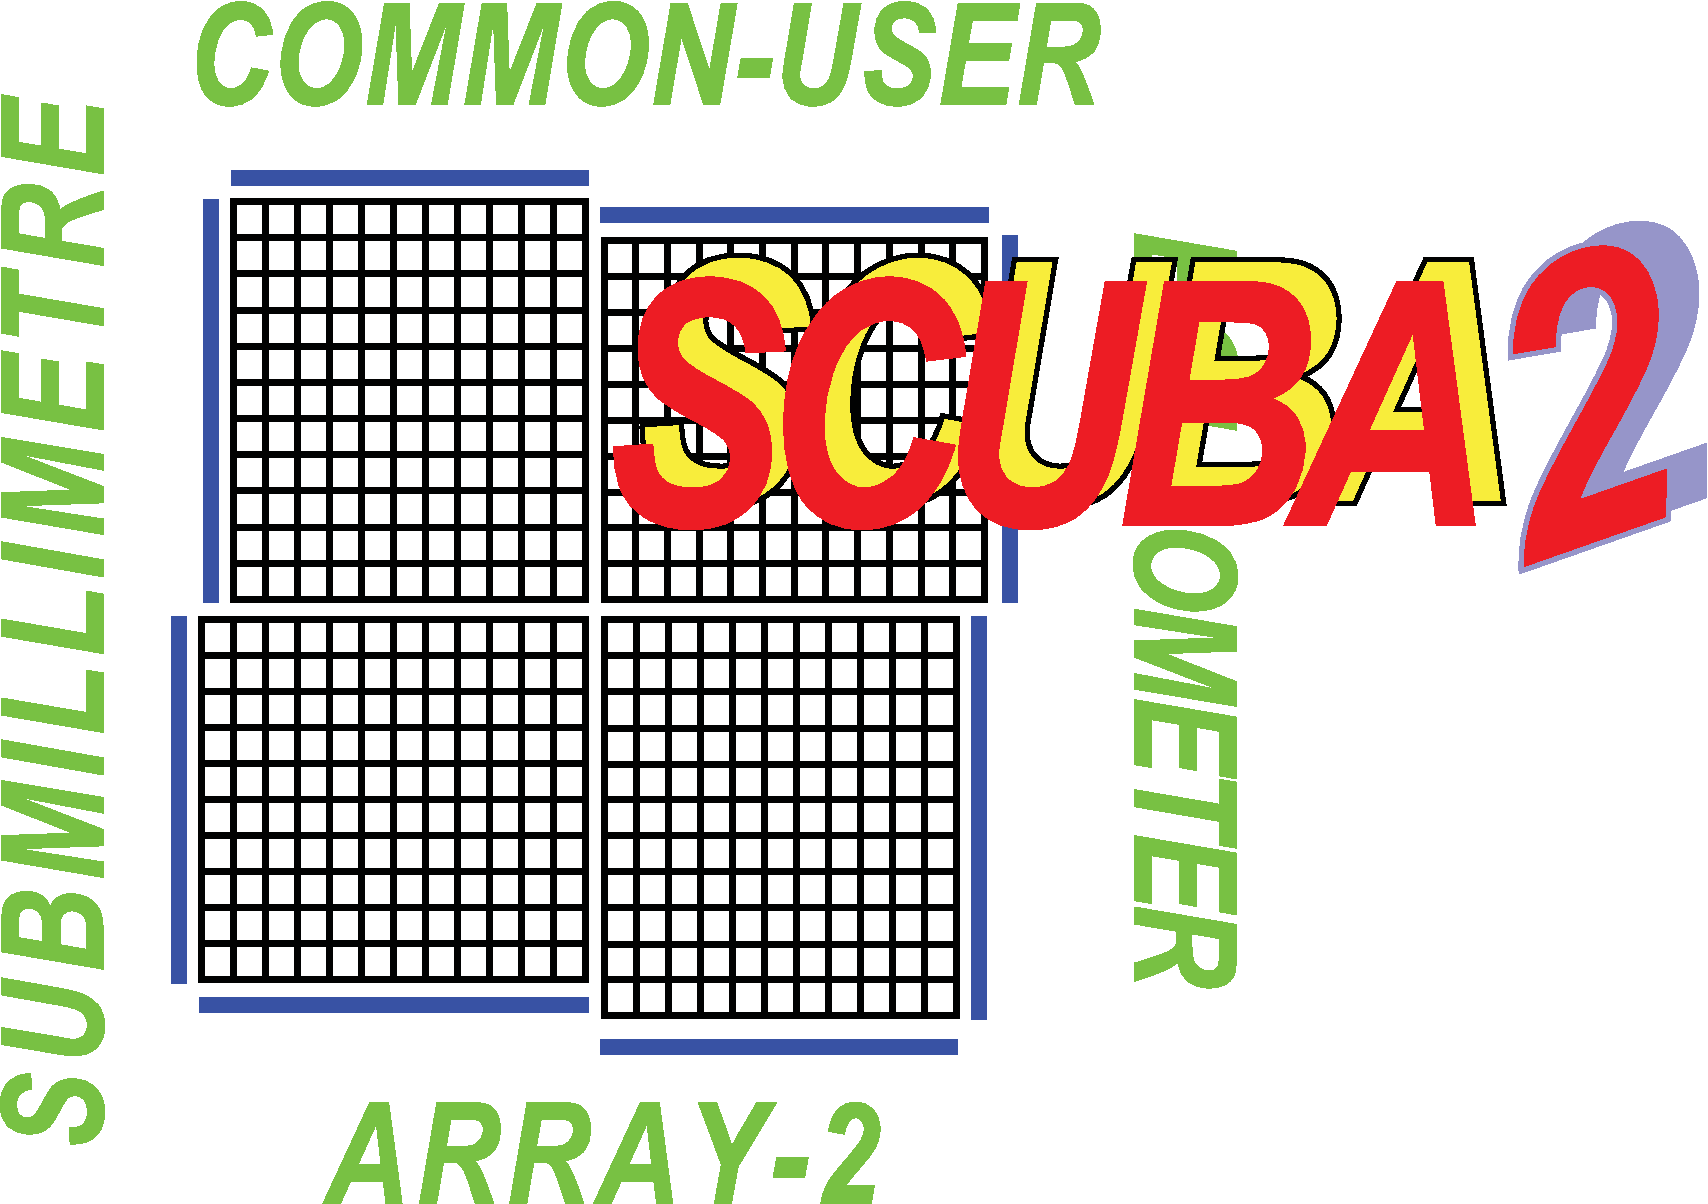
\includegraphics[scale=0.3]{sc19_logo}
\end{center}
% ? End of picture

% ? Heading for abstract if used.
   \vspace{10mm}
   \begin{center}
      {\Large\textbf{Abstract}}
   \end{center}
% ? End of heading for abstract.
\end{latexonly}

%  HTML documentation header.
%  ==========================
\begin{htmlonly}
   \xlabel{}
   \begin{rawhtml} <H1> \end{rawhtml}
      \stardoctitle\\
      \stardocversion\\
      \stardocmanual
   \begin{rawhtml} </H1> <HR> \end{rawhtml}

% ? Add picture here if required for the hypertext version.
%   e.g. \includegraphics[scale=0.7]{filename.ps}
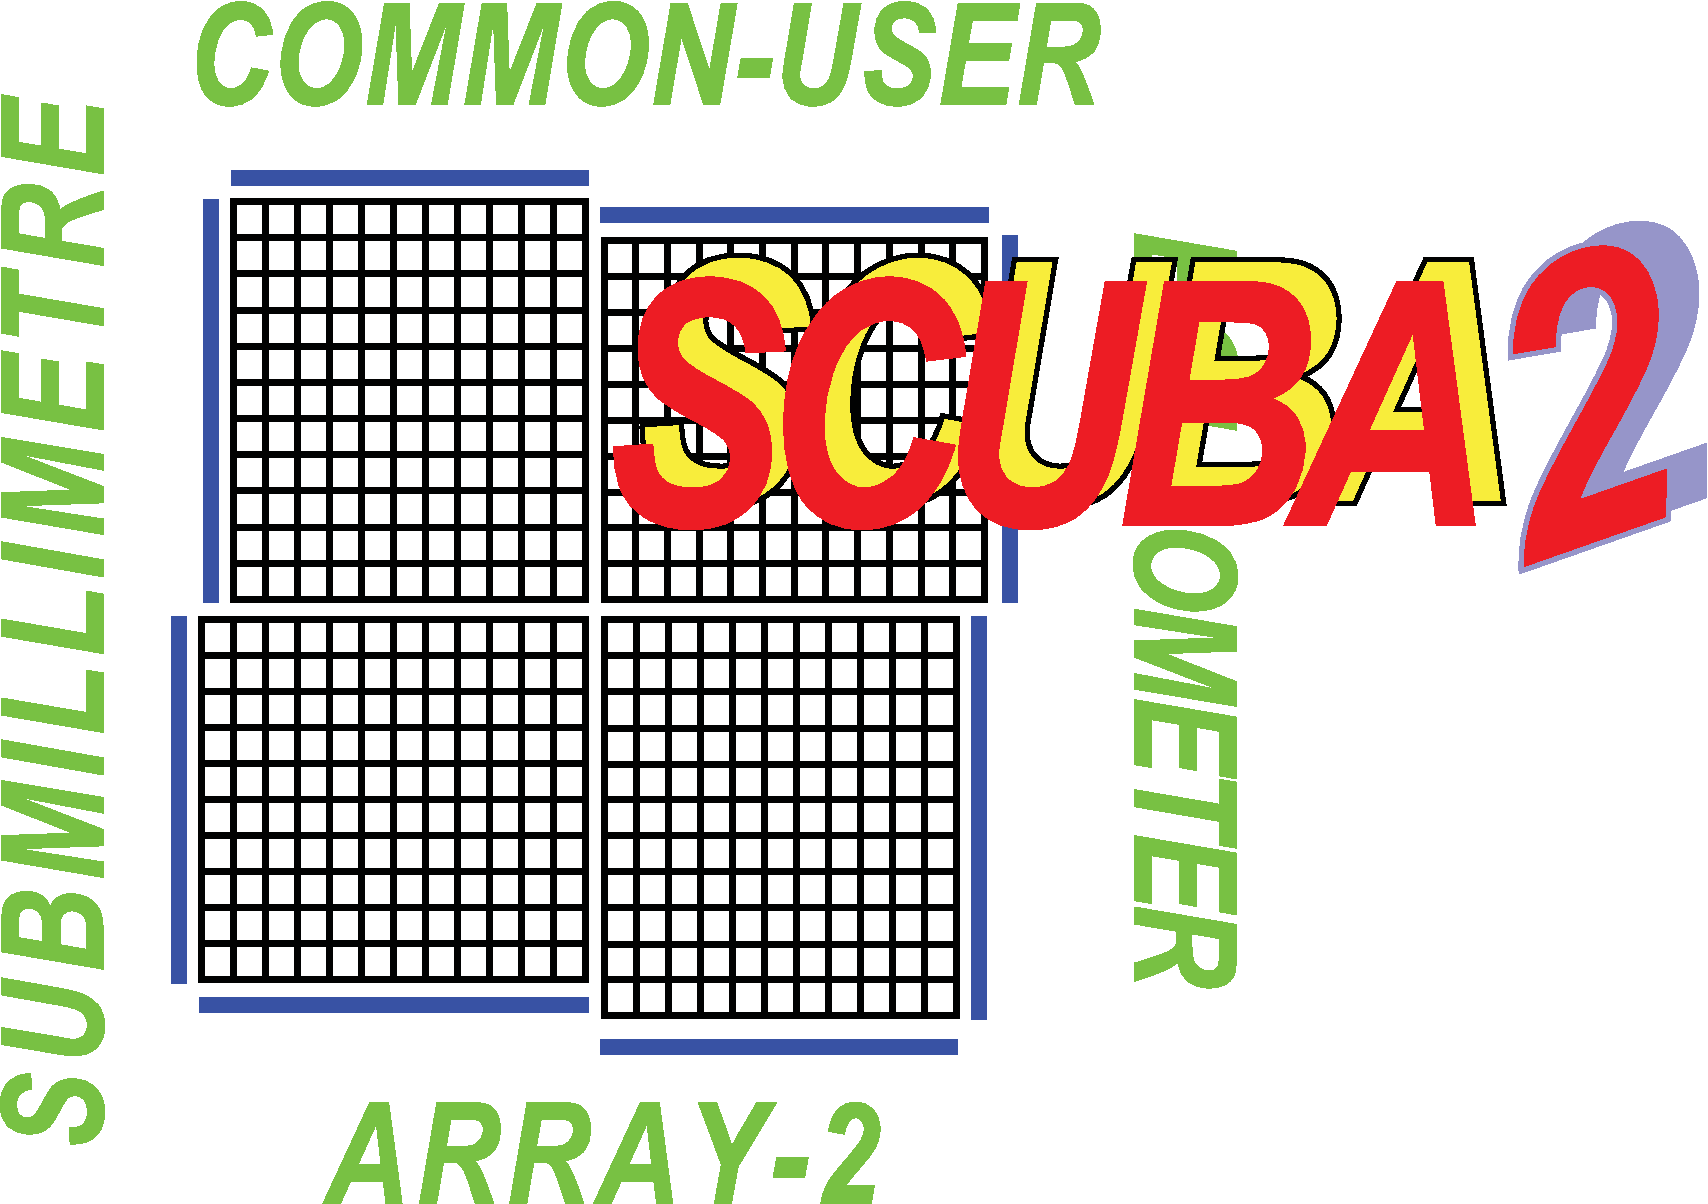
\includegraphics[width=2.0in]{sc19_logo}
% ? End of picture

   \begin{rawhtml} <P> <I> \end{rawhtml}
   \stardoccategory\ \stardocnumber \\
   \stardocauthors \\
   \stardocdate
   \begin{rawhtml} </I> </P> <H3> \end{rawhtml}
      \htmladdnormallink{University of British Columbia}
                        {http://www.ubc.ca} \\
      \htmladdnormallink{Science \& Technology Facilities Council}
                        {http://www.scitech.ac.uk} \\
   \begin{rawhtml} </H3> <H2> \end{rawhtml}
      \htmladdnormallink{Starlink Project}{http://www.starlink.ac.uk/}
   \begin{rawhtml} </H2> \end{rawhtml}
   \htmladdnormallink{\htmladdimg{source.gif} Retrieve hardcopy}
      {http://www.starlink.ac.uk/cgi-bin/hcserver?\stardocsource}\\

%  HTML document table of contents.
%  ================================
%  Add table of contents header and a navigation button to return to this
%  point in the document (this should always go before the abstract \section).
  \label{stardoccontents}
  \begin{rawhtml}
    <HR>
    <H2>Contents</H2>
  \end{rawhtml}
  \htmladdtonavigation{\htmlref{\htmladdimg{contents_motif.gif}}
        {stardoccontents}}

% ? New section for abstract if used.
  \section{\xlabel{abstract}Abstract}
% ? End of new section for abstract
\end{htmlonly}

% -----------------------------------------------------------------------------
% ? Document Abstract. (if used)
%  ==================
\stardocabstract
% ? End of document abstract

% -----------------------------------------------------------------------------
% ? Latex Copyright Statement
%  =========================
\begin{latexonly}
\newpage
\vspace*{\fill}
\stardoccopyright
\end{latexonly}
% ? End of Latex copyright statement

% -----------------------------------------------------------------------------
% ? Latex document Table of Contents (if used).
%  ===========================================
  \newpage
  \begin{latexonly}
    \setlength{\parskip}{0mm}
    \tableofcontents
    \setlength{\parskip}{\medskipamount}
    \markboth{\stardocname}{\stardocname}
  \end{latexonly}
% ? End of Latex document table of contents
% -----------------------------------------------------------------------------

\cleardoublepage
\renewcommand{\thepage}{\arabic{page}}
\setcounter{page}{1}

\section{\xlabel{introduction}Introduction}

The Submillimetre Common User Bolometer Array-2 (SCUBA-2) is a
large-format bolometer camera for the 15-m James Clerk Maxwell
Telescope, designed to produce simultaneous continuum images with
central wavelengths at 450 and 850\,\micron.

The purpose of this guide is to help SCUBA-2 users become familiar
with the basic facilities for analyzing and visualizing data using
\smurf\ \cite{smurf}, and the \starlink\ packages \Kappa \cite{kappa},
and \gaia \cite{gaia}.  This guide is {\em not} aimed at users of the
polarimeter (POL-2) or Fourier transform spectrometer (FTS-2), neither of
which are operational at the time of writing.

A brief description of raw SCUBA-2 data is given in
Section~\ref{sec:data}. Section~\ref{sec:visual} demonstrates how to
visualize SCUBA-2 data, interspersed with some simple worked examples
of interactive data-reduction techniques. The end goal of this section
is {\em not} to produce a final science-grade map; rather to give the
user a feel for the types of artifacts and data reduction steps
required to make a useful image. The best way to make an image from
SCUBA-2 data is to use the Dynamic Iterative Map-Maker. This one-line
command and a subset of its control parameters are described in
Section~\ref{sec:maps}. For the user that wishes only to produce maps
in as little time as possible, jump straight to this latter section.

Note that a number of the examples in this document use real data that
are distributed with this \starlink\ release. They may be found in

\begin{myquote}
\begin{verbatim}
$STARLINK_DIR/share/smurf/s4a20091214_00015_000*.sdf
\end{verbatim}
\end{myquote}

If you wish to use these data for scientific purposes, explicit
permission must be obtained from the Director of the James Clerk
Maxwell Telescope.

To gain access to \smurf\ tasks (the data reduction package for
SCUBA-2) before proceeding with the examples in this document first
type:

\begin{myquote}
\begin{verbatim}
% smurf


        SMURF commands are now available -- (Version 1.0.0)

        Type smurfhelp for help on SMURF commands.
        Type 'showme sun258' to browse the hypertext documentation.
        Type 'showme sc19' to view the SCUBA-2 map-making cookbook.

\end{verbatim}
\end{myquote}
%

For a more detailed description refer to the comprehensive Starlink
User Note (\xref{\textbf{SUN/258}}{sun258}{}).


\section{\xlabel{data_files}SCUBA-2 Data Files}
\label{sec:data}

The SCUBA-2 data acquisition (DA) system writes data files every
30\,s, one file for each of the $40\times32$ pixel subarrays. In
addition, each observation is preceded and followed by dark
observations. For example, observation 15 on 2009-12-14 of Uranus
produced the following 16 files with the 450\,\micron\ array that was
operational at the time (s4a):

\begin{myquote}
\begin{verbatim}
-rw-r--r-- 1 echapin software  5976576 Jan 17 08:01 s4a20091214_00015_0001.sdf
-rw-r--r-- 1 echapin software 34945536 Jan 17 08:01 s4a20091214_00015_0002.sdf
-rw-r--r-- 1 echapin software 34945536 Jan 17 08:01 s4a20091214_00015_0003.sdf
-rw-r--r-- 1 echapin software 34945536 Jan 17 08:01 s4a20091214_00015_0004.sdf
-rw-r--r-- 1 echapin software 34945536 Jan 17 08:02 s4a20091214_00015_0005.sdf
-rw-r--r-- 1 echapin software 34945536 Jan 17 08:02 s4a20091214_00015_0006.sdf
-rw-r--r-- 1 echapin software 34945536 Jan 17 08:02 s4a20091214_00015_0007.sdf
-rw-r--r-- 1 echapin software 34945536 Jan 17 08:02 s4a20091214_00015_0008.sdf
-rw-r--r-- 1 echapin software 34945536 Jan 17 08:02 s4a20091214_00015_0009.sdf
-rw-r--r-- 1 echapin software 34945536 Jan 17 08:02 s4a20091214_00015_0010.sdf
-rw-r--r-- 1 echapin software 34945536 Jan 17 08:02 s4a20091214_00015_0011.sdf
-rw-r--r-- 1 echapin software 34945536 Jan 17 08:02 s4a20091214_00015_0012.sdf
-rw-r--r-- 1 echapin software 34945536 Jan 17 08:02 s4a20091214_00015_0013.sdf
-rw-r--r-- 1 echapin software 34945536 Jan 17 08:02 s4a20091214_00015_0014.sdf
-rw-r--r-- 1 echapin software 11778560 Jan 17 08:02 s4a20091214_00015_0015.sdf
-rw-r--r-- 1 echapin software  5977600 Jan 17 08:02 s4a20091214_00015_0016.sdf
\end{verbatim}
\end{myquote}

As noted in the introduction, the first two files containing data from
the actual scan of Uranus are included with this \starlink\ release in:
\begin{verbatim}
$STARLINK_DIR/share/smurf/s4a20091214_00015_000*.sdf
\end{verbatim}

\Kappa\ tasks such as \fitslist\ and \ndftrace\ can be used to see the
FITS headers and dimensions of the data. In this example, the first
and last files are dark observations, and all the other files are
produced by a single continuous scan of Uranus. The main data arrays
of each file are cubes, with the first two dimensions enumerating
columns and rows, and the third time slices (sampled at 200\,Hz).

Raw SCUBA-2 data are stored as integers (uncalibrated digitized
units). The \smurf\ task \flatfield\ can be used to scale raw data to
units of pW (double precision floating points) using the results of
measurements of calibrated loads that are stored internally (the HDS
extension is MORE.SCUBA2.FLATCAL). Use the command

\begin{myquote}
\begin{verbatim}
% flatfield 's4d20090107_00007_00*.sdf' '*_flat'
\end{verbatim}
\end{myquote}
%
to produce flat-fielded versions of the files that contain bolometer
data taken during the scan across Uranus, with the dark observations
(1 and 16) automatically filtered out. Note that the single quotes
around the wildcards for the input and output files are necessary
since \starlink\ routines expand them internally, rather than using
the shell. However, it is not generally necessary to use \flatfield\
before proceeding with map-making. \smurf\ will flatfield the data
internally as needed.

\section{\xlabel{time_series}Visualizing data}
\label{sec:visual}

In this section several procedures are described for looking at
SCUBA-2 data, as well as basic data reduction steps that can be run
separately. Working through these examples illustrate some of the
features of SCUBA-2 data, but will not result in a science-grade image
at the end. If you are interested only in making the best possible map
with minimal effort go immediately to Section~\ref{sec:maps}.

\subsection{\xlabel{concat}Concatenating data}

Since SCUBA-2 data for a given subarray are broken into many pieces by
the DA system, it is useful for visualization to first concatenate the
data into single files. The \smurf\ task \concat\ can be used for this
operation. For example,

\begin{myquote}
\begin{verbatim}
% sc2concat 's4a20091214_00015_000*.sdf' './*_con'
\end{verbatim}
\end{myquote}

combines all of the files associated with observation 15 for the s4a
array into a single file called
s4a20091214\_00015\_0002\_con.sdf. \concat\ will automatically filter
out any dark observations, so that the concatenated file contains only
the data taken during the scan across Uranus with the shutter open. It
also applies the flatfield by default, although it can be disabled using
the `noflat' option on the command-line.

\subsection{\xlabel{display_scan}Displaying scan patterns}

The pointing of the telescope throughout a scan (as well as other
state information) is stored in the MORE.SMURF.JCMTSTATE extension of
a data file. The \smurf\ task \jcmtstate\ will convert this
information into a simple ASCII tab separated table:

\begin{myquote}
\begin{verbatim}
% jcmtstate2cat s4d20090107_00007_0002_concat > state.tst
\end{verbatim}
\end{myquote}

\begin{figure}
\begin{center}
\includegraphics{sc19_scan_pattern}
\caption{The telescope positions during observation number 7 on
  20090107. The plot is created by \topcat\ from the output from
\jcmtstate\ plotting the DRA columns against the DDEC column. The pong
scan pattern is clearly visible.}
\label{fig:topcat}
\end{center}
\end{figure}

The `-h' option to \jcmtstate\ can be used to find more information on
the command. In particular, multiple files can be supplied to the
command using standard shell wild cards (not escaped) and for SCUBA-2
data the `--with-mce' option can be used to dump the low-level MCE
header information.

This catalogue can be loaded into \topcat\ for plotting, making sure
that \topcat\ is told that the TST format is to be used for reading.

\begin{myquote}
\begin{verbatim}
% topcat -f tst state.tst
\end{verbatim}
\end{myquote}

An example plot of the scan pattern for this observation generated by
\topcat\ can be seen in Fig.~\ref{fig:topcat}.

\subsection{\xlabel{display_cube}Displaying data cubes}

\begin{figure}
\begin{center}
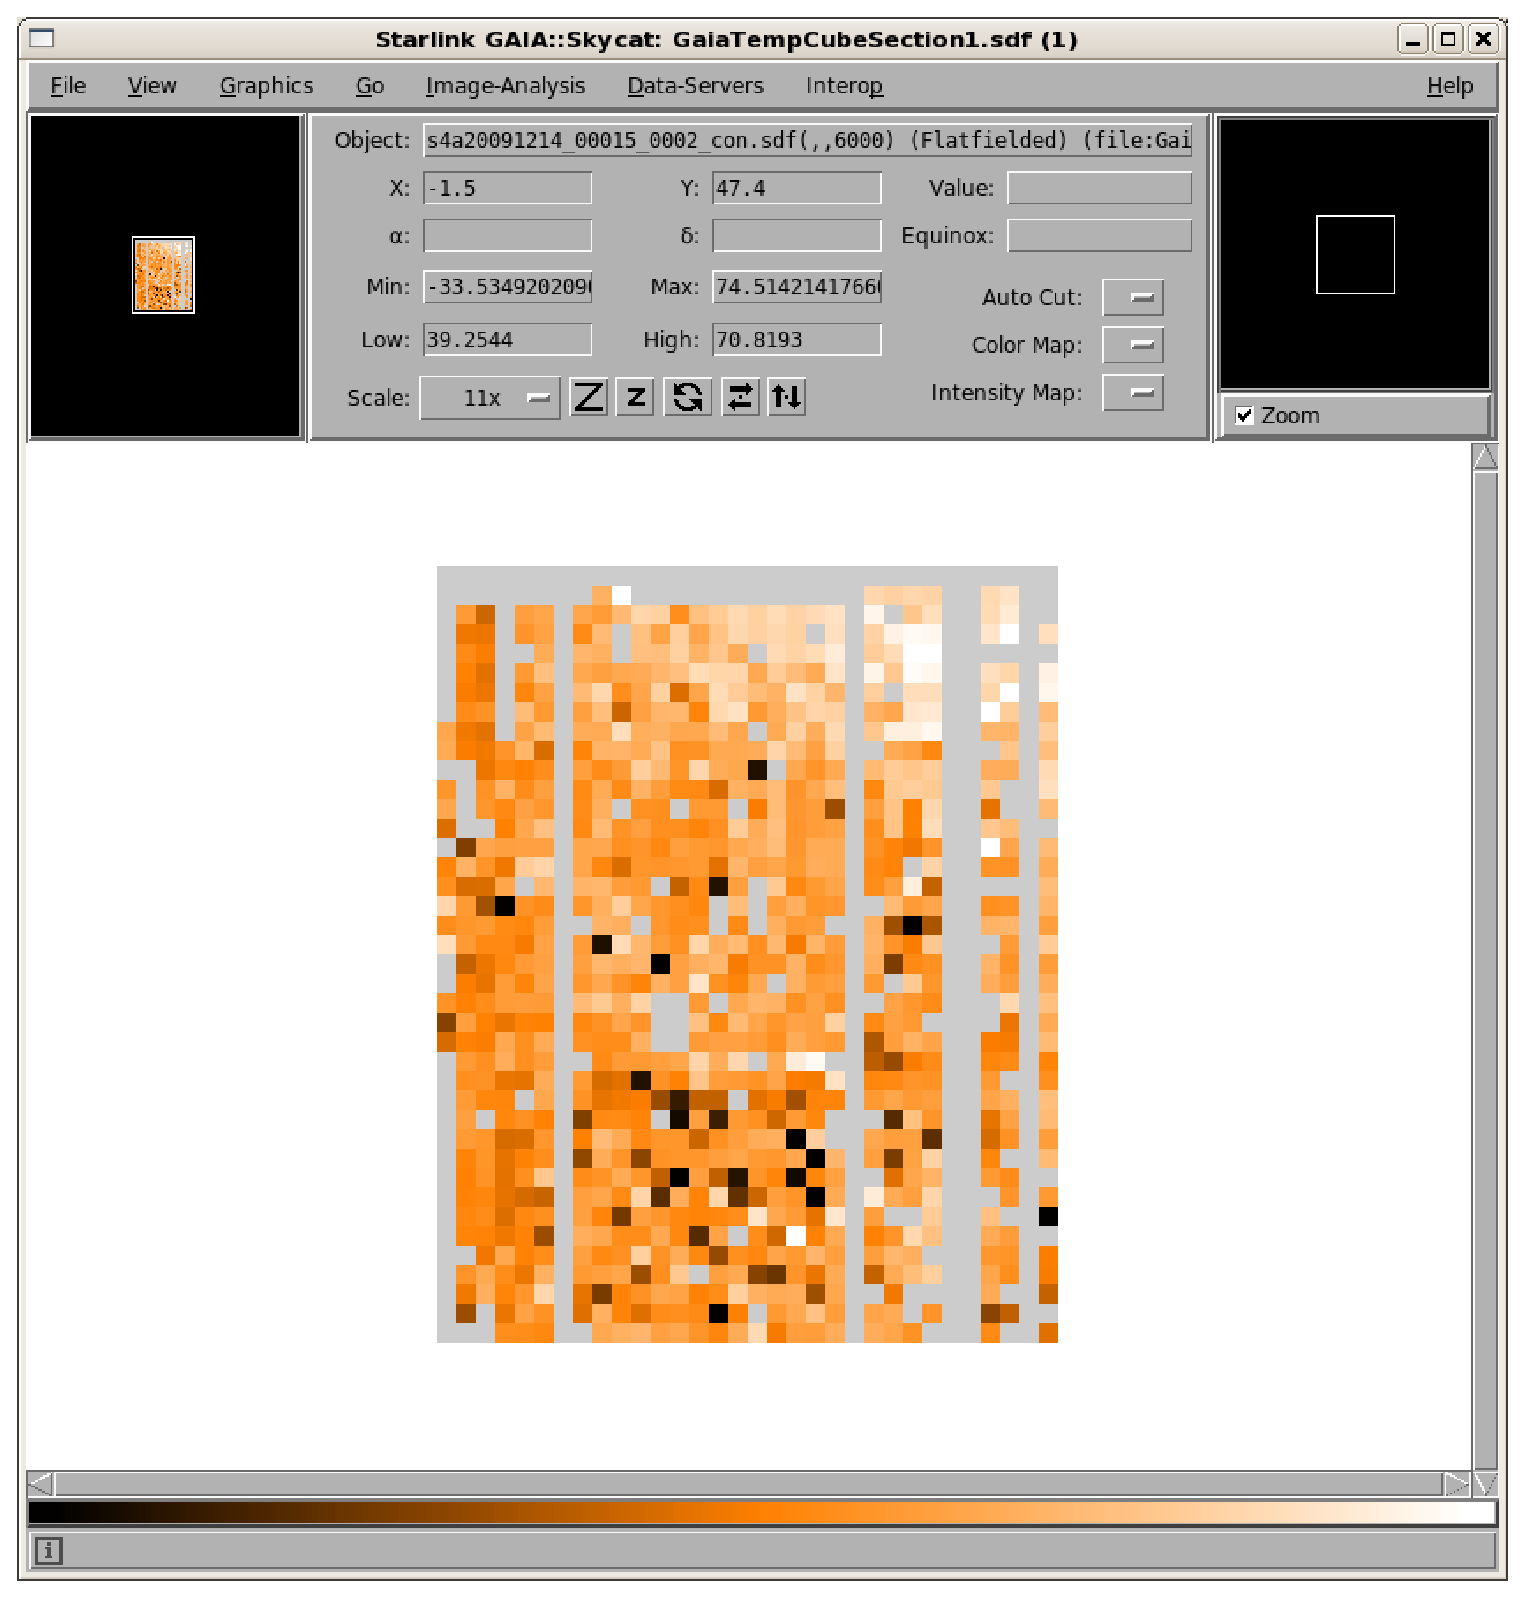
\includegraphics[width=0.61\linewidth]{sc19_gaia_main}\hspace{0.03\linewidth}
\includegraphics[width=0.33\linewidth]{sc19_gaia_sections}
\caption{Initial \gaia\ windows displayed upon loading a data cube
  (with slight modifications to the colour table using options under
  the `View' tab). {\bf Left:} The main window, after clicking the `Z'
  button a number of times to zoom-in, shows a map of detector values
  at a fixed sample in time. Note that these data came from an array
  with a number of broken columns and broken isolated detectors, all
  indicated in grey. {\bf Right:} The `Display image sections of a
  cube' dialogue enables the user to navigate the time dimension. The
  `Index of plane' slider near the top can be used to select different
  time slices, and the main window will automatically update.}
\label{fig:gaia_main}
\end{center}
\end{figure}

The easiest way to visualize the detector time series data is to use
\gaia. Loading in the concatenated file above (combining the two
example files included with this \starlink\ release) produces two
windows (Fig.~\ref{fig:gaia_main}). The main window shows a map of
detector values at a given instant in time. The second window can be
used to navigate the time axis: by moving the `Index of plane' slider
in the `Display image sections of a cube' dialogue, different time
slices may be selected, with the main \gaia\ window updating
automatically.

For this concatenated data file (1\,min. in total as it is the
combination of two 30\,s files), each detector has a large offset
relative to its neighbours as well as relative to any smaller
time-varying signals, which means that little difference can be seen
by moving the slider. However, \gaia\ can produce an automatically
scaled plot of the time-series for an individual detector by simply
clicking on it in the main window. For example, clicking on the
detector at (13,23) spawns the `Spectral plot' window shown in
Fig.~\ref{fig:gaia_spec} for a single detector. Clicking on other
detectors over-writes the plot of the original detector in the same
window. Looking at the vertical axis range on the left, the mean
levels clearly vary significantly from detector to detector, although
the time-varying component of the signals are quite similar.

\begin{figure}
\begin{center}
\includegraphics[width=0.7\linewidth]{sc19_gaia_spec}
\caption{The `Spectral Plot' window is spawned automatically once a
  detector is clicked in the main window, such as (13,23) in this
  example, displaying its time-varying signal. The vertical red line
  indicates the time slice that is currently selected in the `Display
  image sections of a cube' dialogue. The regular pattern with a
  period of about 30 seconds (in this particular case) is slow
  baseline drift correlated with variations in the SCUBA-2 fridge
  temperature. The green-circled narrow spike is produced by the
  detector crossing Uranus. Usually astronomical signals are not
  readily visible in raw time-series plots such as these as they are
  relatively much fainter. It is also worth noting that the `gaps'
  apparent near the start of the time series, and at $\sim34$\,s are
  simply artifacts of the plotting software re-sampling the data to
  the resolution of the display (zooming-in to these regions using the
  `Lower index' and `Upper index' sliders in the `Display image
  sections of a cube' dialogue followed by a click on `Re-extract' to
  update the plot demonstrates this).  }
\label{fig:gaia_spec}
\end{center}
\end{figure}

\subsection{\xlabel{regrid_map}Regridding data into a map}

A `naive' map can be made from a data cube using the \smurf\ \makemap\
task. The following will produce a map directly from the raw
concatenated data by re-gridding it into a pixelated map:

\begin{myquote}
\begin{verbatim}
% makemap s4a20091214_00015_0002_con.sdf uranus method=rebin
\end{verbatim}
\end{myquote}

The \makemap\ task automatically scales the bounds of the image to
encompass all of the data. The output map here is called `uranus.sdf',
and the pixel scale is 2~arcsec on a side by default at 450\,\micron\
(although this can be changed using the `pixsize=$x$' option on the
command-line, where $x$ is in arcsec). Since we already know that
relative detector offsets are large in these data, it is unsurprising
that nothing can really be seen in the resulting image with \gaia.

\begin{figure}
\begin{center}
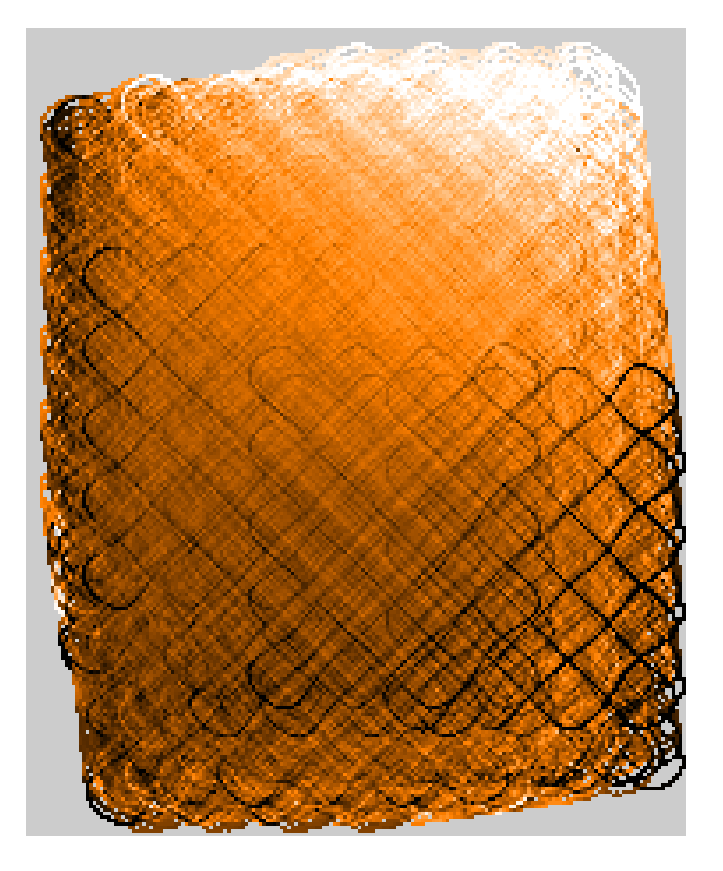
\includegraphics[width=0.5\linewidth]{sc19_rawmap}
\caption{Map produced from raw data of a scan across Uranus. The
  image is completely dominated by noise in the relative signal
  offsets of each bolometer, and no astronomical signal can be
  seen. The scan (a Curvy PONG) can clearly be seen as a repetitive
  `waffle' pattern in the image.}
\label{fig:rawmap}
\end{center}
\end{figure}

\subsection{\xlabel{clean}Cleaning data}

The previous examples illustrate the need for some kind of data
cleaning before there is any hope of seeing astronomical sources. A
useful \smurf\ task for time-domain data processing is \clean, which
can perform several different steps controlled by a range of
parameters. Note that all of the algorithms available to \clean\ are
also accessible within the DIMM (Section~\ref{sec:maps}), so in
practice the user does not issue this command directly before making
the final map.

\subsubsection{\xlabel{clean_average}Removing detector averages and DC Steps}

The following will remove a 0th-order polynomial (the mean) from each
detector time stream, storing the cleaned data in a file called
`clean.sdf':

\begin{myquote}
\begin{verbatim}
% sc2clean s4a20091214_00015_0002_con.sdf clean \
     config="order=0"
\end{verbatim}
\end{myquote}

\begin{figure}
\begin{center}
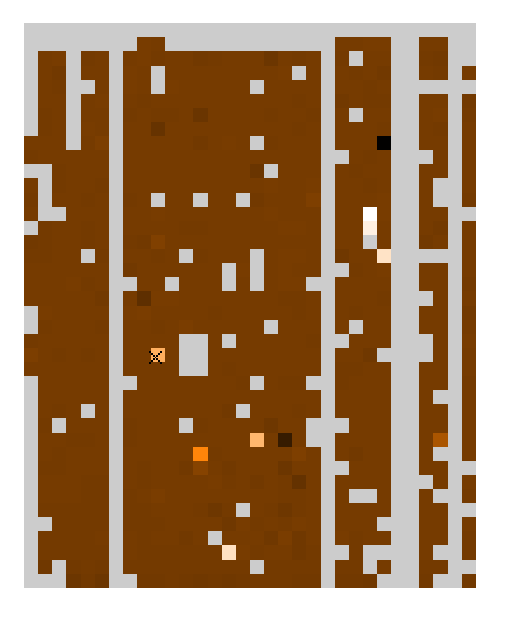
\includegraphics[width=0.5\linewidth]{sc19_array_mean}
\includegraphics[width=0.9\linewidth]{sc19_dcstep}
\caption{{\bf Top:} \gaia\ plot of the array signal at time slice 1
  after using \clean\ to remove the mean of each detector signal
  (clean.sdf). The LOW and HIGH data values for this intensity plot
  are $-1.7171$\,pW and $+5.50352$\,pW, respectively. Most of the
  working detectors (not grey) now have approximately the same signal
  range (approximately $\pm 0.1$\,pW), and therefore have nearly the
  same colour (brown). However, there are several outliers: for
  example, the orange pixel with an `x' at (10,17). {\bf Bottom:} The
  time series for detector (10,17) showing the presence of a large
  level change, or `DC Step' near 29\,s.}
\label{fig:array_mean}
\end{center}
\end{figure}

This operation results in bolometer data that lie primarily in the
range $\pm 0.1$\,pW, except for a handful of outliers as shown in
Fig.~\ref{fig:array_mean}. In these cases there have been large level
changes, or `DC Steps' while the data were being acquired. These can
be identified and repaired using some extra parameters to \clean:

\begin{myquote}
\begin{verbatim}
% sc2clean s4a20091214_00015_0002_con.sdf clean2 \
   config='"order=0,dcfitbox=400,dcthresh=5,fillgaps=1"'
\end{verbatim}
\end{myquote}

The parameters starting with `dc' indicate that \clean\ should look
for steps in the data in excess of 200-$\sigma$ comparing two
consecutive boxcar averages of length 50 samples.  Finally,
`fillgaps' indicates that the data range around the identified steps
($\pm 50$ samples in this case) should be replaced with a constrained
(smooth) realization of noise to avoid introducing spikes into the
data stream (these short ranges are ultimately ignored when producing
final maps). A map produced from `clean2.sdf' is shown in
Fig.~\ref{fig:map_dc_mean}.

\begin{figure}
\begin{center}
\includegraphics[width=0.5\linewidth]{sc19_map_mean_dc}
\caption{Map produced from clean2.sdf in which DC steps have been
  repaired and the detector means have been subtracted. There are
  still many artifacts in the data, but now Uranus is visible.}
\label{fig:map_dc_mean}
\end{center}
\end{figure}

The command line can get long, so it is also possible to write the
configuration parameters into a text file and specify the text file
for CONFIG using the standard group notation:

\begin{myquote}
\begin{verbatim}
% sc2clean s4a20091214_00015_0002_con.sdf clean2 \
   config=^myconfig.lis
\end{verbatim}
\end{myquote}

An example config file containing the default values for each item
can be found in \verb|${SMURF_DIR}/smurf_sc2clean.def|.

\subsubsection{\xlabel{movie}Watching a movie}

\gaia\ has the ability to animate the display of a data cube. We will
use this feature to make a `movie' of the array data. Load
`clean2.sdf' from the previous step into \gaia\. In the `Display image
sections of a cube' dialogue, switch from the `Spectrum' to the
`Animation' tab approximately half-way down.  Set `Delay' to 10
milliseconds (the smallest value), `Step' to 5 (such that it only
shows 1 in every 5 frames), and click the `On' button next to
`Looping'. Finally, click `Start', and an animation of the data cube
will be shown in the main \gaia\ window. The dominant signal is a
gradual variation in the average value of all of the detectors in
unison. This {\em common mode} signal is produced through a
combination of SCUBA-2 fridge temperature variations, sky noise,
telescope motion, and other drifts in the individual detectors. At
times it is also (just barely) possible to see Uranus itself as the
array scans.

\subsubsection{\xlabel{fftfilter}Frequency-domain filtering}

\clean\ can also perform frequency domain filtering on the
detectors. In order for this to work properly, the data must first be
apodized (smoothly rolled-off to 0 at the beginning and end), and some
padding added to the beginning and end, to avoid ringing. The
following steps will concatenate the raw data files together adding
padding at the beginning and end, and then apodize and filter the
single large file.

\begin{figure}
\begin{center}
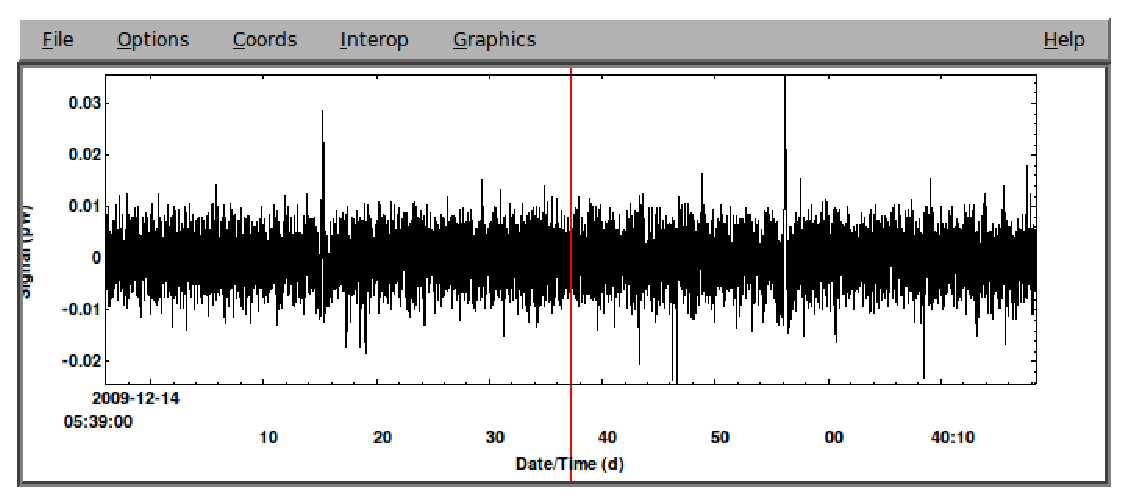
\includegraphics[width=\linewidth]{sc19_spec_filt} \\
\vspace{0.3in}
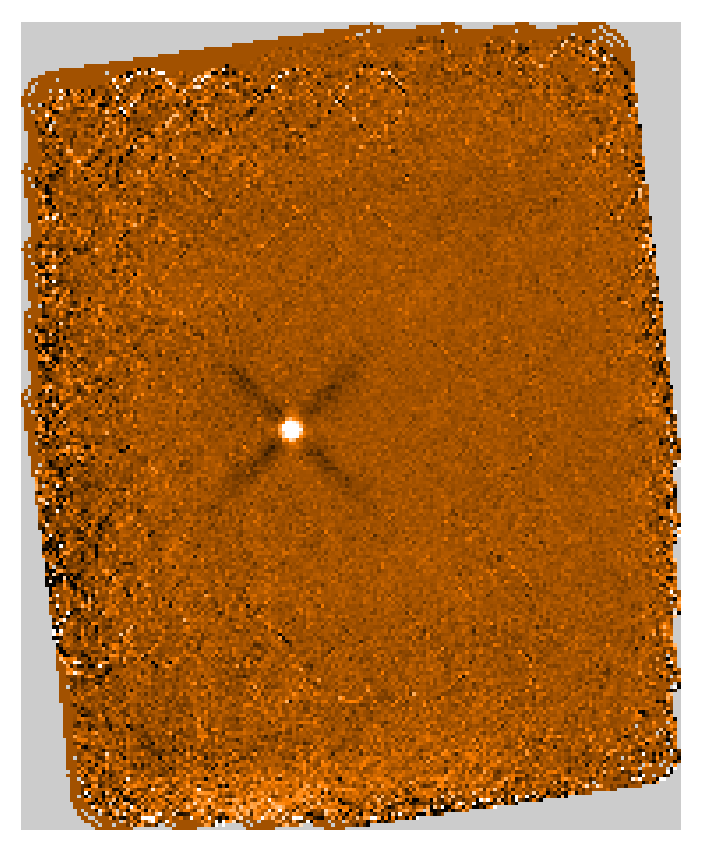
\includegraphics[width=0.5\linewidth]{sc19_map_highpass}
\caption{High-pass filtered data (clean3.sdf). {\bf Top:} The time
  series for a single detector (13,23). Comparing with the un-filtered
  data in Fig.~\ref{fig:gaia_spec} the positive spikes produced by
  Uranus are now much more apparent. {\bf Bottom:} a map produced from
  these cleaned and filtered data. The brightness of Uranus compared
  to the noise is now much more significant than in
  Fig.~\ref{fig:map_dc_mean}, but the filtering has caused negative
  ringing around source crossing in the time series which appear as
  negative dips in the map along the scan directions (negative cross
  around the source).}
\label{fig:highpass}
\end{center}
\end{figure}

\begin{myquote}
\begin{verbatim}
% sc2concat 's4a20091214_00015_000?.sdf' './*_con2' padstart=1000 \
padend=1000

Out of 2 input files, 0 were darks and 2 were not darks
Processing data from instrument 'SCUBA-2' for object 'URANUS' from the
following observation  :
  20091214 #15 scan

% sc2clean s4a20091214_00015_0002_con2.sdf clean3 \
   config=^${STARLINK_DIR}/share/smurf/sc19_clean3.lis

Processing data from instrument 'SCUBA-2' for object 'URANUS' from the
following observation  :
  20091214 #15 scan

\end{verbatim}
\end{myquote}

where the text file contains the following configuration options:

\begin{myquote}
\begin{verbatim}
order=0
dcfitbox=400
dcthresh=5
dcmedianwidth=40
fillgaps=1
apod=1000
filt_edgehigh=0.5
\end{verbatim}
\end{myquote}

When concatenating the data using \concat\ an additional 1000 samples
at the start and end of the data have been added as padding. The call
to \clean\ has done several things: removed the mean value of each
detector; corrected DC steps; apodized over a range of 1000 samples;
and finally performed a high-pass filter with a hard lower cutoff
frequency of 0.5\,Hz.

Fig.~\ref{fig:highpass} shows the filtered bolometer signal for
(13,23), as well as a map produced from the data. The filtering has
significantly improved the noise properties of the map compared with
Fig.~\ref{fig:map_dc_mean}, but the filtering has now introduced
negative ringing around the source which results in a negative cross
pattern along the scan directions.

\subsection{\xlabel{pspec}Detector power-spectra}

The frequency-domain power spectra of SCUBA-2 detectors can be
produced with the \smurf\ task \fft. Using the padded, concatenated
data `s4a20091214\_00015\_0002\_con2.sdf' from the previous step, use the
following commands:

\begin{myquote}
\begin{verbatim}

% sc2clean s4a20091214_00015_0002_con2 clean4 \
   config='"^${STARLINK_DIR}/share/smurf/sc19_clean3.lis,filt_edgehigh=0"'

Processing data from instrument 'SCUBA-2' for object 'URANUS' from the
following observation  :
  20091214 #15 scan

% sc2fft clean4 pspec power=true

Processing data from instrument 'SCUBA-2' for object 'URANUS' from the
following observation  :
  20091214 #15 scan

Found 1 continuous chunk
SC2FFT: power spectrum requested so setting POLAR=TRUE

\end{verbatim}
\end{myquote}

As in the previous examples we have used \clean\ to fix DC steps,
remove the mean, and apodize the data (to suppress ringing when we
take the FFT). However, we omit the high-pass filtering, since the
goal now is to see what the bolometer noise looks like. Since there is
no \starlink\ standard format for storing complex values, \fft\ uses
its own format: a 4-dimensional array, with the first two axes
indicating detector row and column, the third axis frequency, and the
final axis contains the real and imaginary parts of each Fourier
coefficient. By setting `power=true' it switches to polar form, such
that the first element of the 4th array axis stores the square of the
amplitudes, and the second element stores the arguments (phases) of
each Fourier coefficient. As with the time series data, \gaia\ may
then be used to view the data cube. The difference is that we now
specify a subset of the data so that the 3rd axis of the cube is the
array of squared Fourier amplitudes for each detector, and ignore the
phases (i.e. we observe only the 1st elements along the 4th axis):

\begin{myquote}
\begin{verbatim}
% gaia 'pspec(,,,1)'
\end{verbatim}
\end{myquote}

It is then possible to click on each detector to display its power
spectrum. Once the `Spectral plot' window has been spawned, it will
also be necessary to modify the axis displays. Select
`Options'$\rightarrow$`Positive~Y~Only', and
`Options'$\rightarrow$`Log~Y~Axis'. Similarly, select the
corresponding settings for the `X' axis. Fig.~\ref{fig:pspec} shows
the power spectrum of detector (13,23), with a $1/f$ knee apparent
just below 1\,Hz.

\begin{figure}
\begin{center}
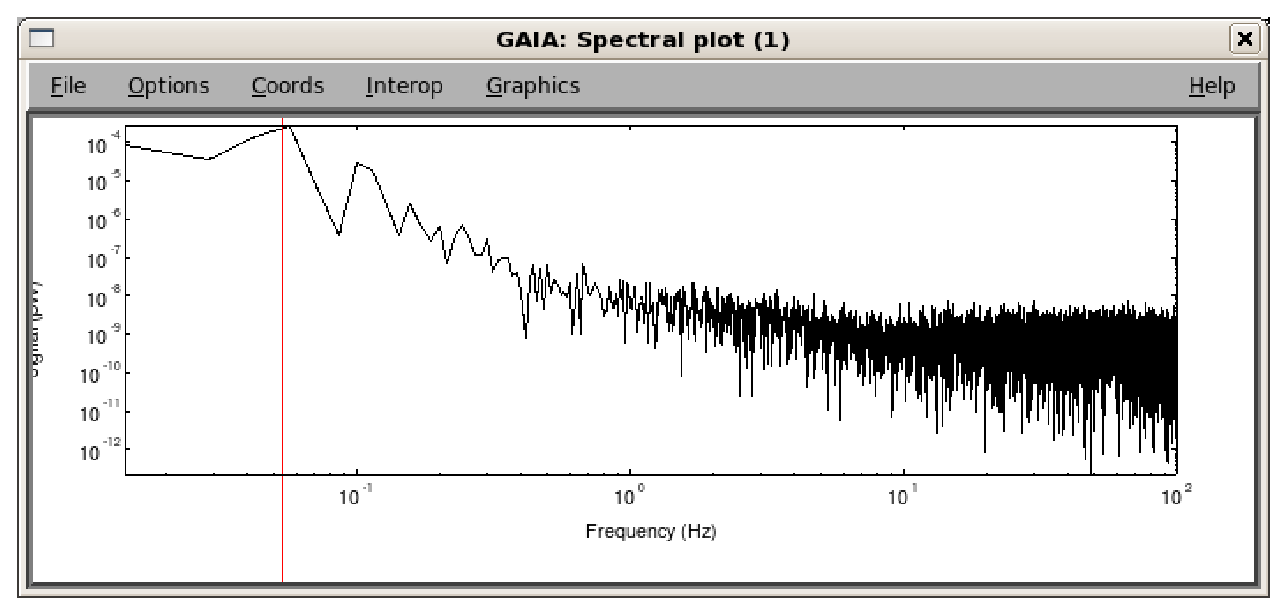
\includegraphics[width=\linewidth]{sc19_pspec}
\caption{The power spectrum of bolometer (13,23) produced by the
  \smurf\ task \fft. In this particular case the noise looks white
  above a $1/f$ knee just below 1\,Hz. The red line simply indicates
  the frequency slice currently being displayed in the main \gaia\
  window (not shown).}
\label{fig:pspec}
\end{center}
\end{figure}

\subsection{\xlabel{quality}Data quality flagging}

NDF files manipulated by \smurf\ use the standard \starlink\ named
Quality mechanism (see discussion in \xref{Masking, Bad Values, and
  Quality}{sun95}{se_masking}). Quality itself is stored as an 8-bit
integer for each sample in a data file, and each bit can reflect a
different condition. For example, the following will indicate the
number of samples flagged by \clean\ when producing `clean4.sdf' in
the previous example:

\begin{myquote}
\begin{verbatim}
% kappa


     KAPPA commands are now available -- (Version 1.12-1)

     Type kaphelp for help on KAPPA commands.
     Type 'showme sun95' to browse the hypertext documentation.

     NOTE, several applications have had major changes made to their
     parameter lists. See the 'Release Notes' section of SUN/95 for
     details.



% showqual clean4 count
  BADDA           (bit 1) - "Set iff a sample is flagged by the DA" (4416000)
  BADBOL          (bit 2) - "Set iff all data from bolo to be ignored" (5194000)
  DCJUMP          (bit 3) - "Set iff a DC jump is present" (25497)
  PAD             (bit 4) - "Set iff data are padding" (2560000)
  APOD            (bit 5) - "Set iff data are apodized/boundary" (5120000)
\end{verbatim}
\end{myquote}

The `count' supplied to \showqual\ indicates that the total number of
occurences of each Quality flag in the data should be counted and
displayed.  This example shows that 4416000 samples in total were
flagged `\texttt{BADDA}' by the data acquisition system. Since each
bolometer produced about 14000 samples (including 2000 for padding),
this corresponds to 4416000/12000 $\sim$ 368 detectors that were not
operational (out of 1280). Similarly, $1280 \,\mathrm{bolometers} \times 2000 =
2560000$ samples flagged as padding, {\texttt PAD}. Finally, the
apodization ({\texttt APOD}) is flagged over the same sample length as
the padding, but then that same amount again is flagged beyond this
region to avoid including any ringing in the final map (i.e. $2560000
\times 2 = 5120000$).

During map-making flagged samples will not be used and by default they
will be hidden from view of all Starlink tools. However, if you wish
to see the data that was flagged you can use the \Kappa\ task \setbb\
command to enable a particular flag or turn them all off.

\begin{myquote}
\begin{verbatim}
% setbb clean4 0
\end{verbatim}
\end{myquote}

will disable quality and make visible all the underlying data.

Additionally, the \Kappa\ task \qualtobad\ may be used to
permanently convert samples with given quality bits to a {\em magic\/} or {\em
  invalid\/} value. For example:

\begin{myquote}
\begin{verbatim}
% qualtobad clean4 badmasked pad
\end{verbatim}
\end{myquote}
%
will set all of the samples during the first and last 1000 time
slices, where the data were padded, to the magic value.  If
`badmasked' is subsequently viewed with \gaia, none of those portions
of the data will be visible.

\section{\xlabel{maps}Dynamic Iterative Map-Making}
\label{sec:maps}

Rather than manually cleaning the data by hand and then re-gridding it
all at the end, we can instead do everything in one go using the
\smurf\ Dynamic Iterative Map-Maker (DIMM).

The DIMM is enabled using the \texttt{method=iterate} switch to the
\makemap\ task. In the following example we will produce a map of
Uranus using the test data supplied with this \starlink\ distribution
in {\texttt \$STARLINK\_DIR/share/smurf/s4a20091214\_00015\_000*.sdf}. All
of the settings for the DIMM are stored in the configuration file
`\texttt{dimmconfig.lis}'. In this example we will use the default
configuration file that is installed in the \starlink\ tree, which is
fully described in the \makemap\ documentation. A local copy can be
made and altered if desired. The following command invokes the DIMM to
produce the image shown in Fig.~\ref{fig:itermap} with 2\,arcsec
pixels:

\begin{myquote}
\begin{verbatim}
% makemap '$STARLINK_DIR/share/smurf/s4a20091214_00015_000?.sdf' uranus 2 \
method=iterate config=^$STARLINK_DIR/share/smurf/dimmconfig.lis

Out of 2 input files, 0 were darks and 2 were not darks
Processing data from instrument 'SCUBA-2' for object 'URANUS' from the
following observation  :
  20091214 #15 scan

MAKEMAP: Map-maker will use 12840 MBytes of memory

   Output sky coordinates are (RA,Dec) offsets from the (moving)
   telescope base position, which started at (RA,Dec) = (23:34:38.6,
-3:33:57).

   Projection parameters used:
      CRPIX1 = 0
      CRPIX2 = 0
      CRVAL1 = 0 ( DRA = 0:00:00.000 )
      CRVAL2 = 0 ( DDec = 0:00:00.00 )
      CDELT1 = -0.000555555555555556 ( -2 arcsec )
      CDELT2 = 0.000555555555555556 ( 2 arcsec )
      CROTA2 = 0

   Output map pixel bounds: ( -74:112, -112:116 )

   Output map WCS bounds:
        Right ascension offset: -0:00:14.867 -> 0:00:10.067
        Declination offset: -0:03:47.00 -> 0:03:51.00

smf_iteratemap: Iterate to convergence (max 5)
smf_iteratemap: Stopping criteria is a change in chi^2 < 0.001
smf_iteratemap: Continuous chunk 1 / 1 =========
smf_iteratemap: Iteration 1 / 5 ---------------
smf_iteratemap: Pre-conditioning chunk
smf_iteratemap: Calculate time-stream model components
smf_iteratemap: Rebin residual to estimate MAP
smf_iteratemap: Will calculate chi^2 next iteration
smf_iteratemap: Calculate ast
smf_iteratemap: Iteration 2 / 5 ---------------
smf_iteratemap: Calculate time-stream model components
smf_iteratemap: Rebin residual to estimate MAP
smf_iteratemap: *** CHISQUARED = 1.29869194479688 for chunk 1
smf_iteratemap: Calculate ast
smf_iteratemap: Iteration 3 / 5 ---------------
smf_iteratemap: Calculate time-stream model components
smf_iteratemap: Rebin residual to estimate MAP
smf_iteratemap: *** CHISQUARED = 1.28393317451548 for chunk 1
smf_iteratemap: *** change: -0.0147587702814003
smf_iteratemap: Calculate ast
smf_iteratemap: Iteration 4 / 5 ---------------
smf_iteratemap: Calculate time-stream model components
smf_iteratemap: Rebin residual to estimate MAP
smf_iteratemap: *** CHISQUARED = 1.28363571374134 for chunk 1
smf_iteratemap: *** change: -0.000297460774144831
smf_iteratemap: Calculate ast
smf_iteratemap: ****** Completed in 4 iterations
smf_iteratemap: ****** Solution CONVERGED
\end{verbatim}
\end{myquote}

\begin{figure}
\begin{center}
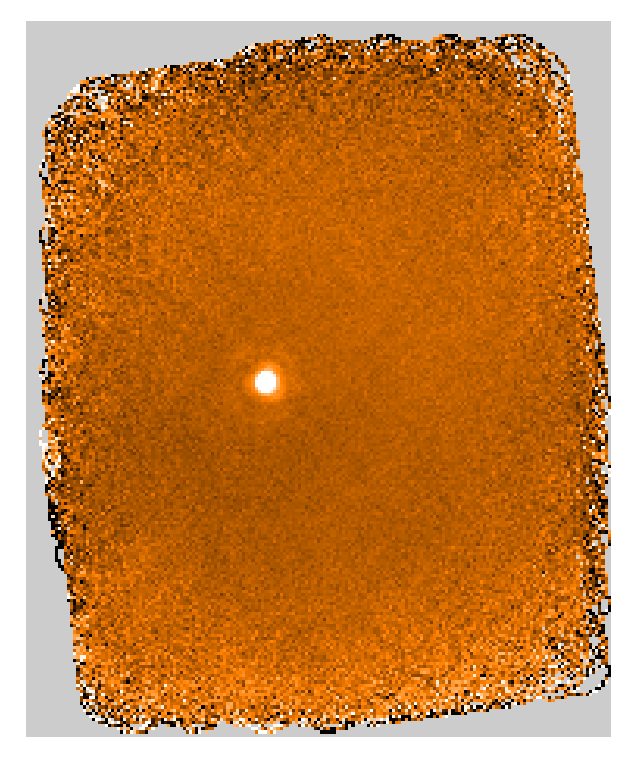
\includegraphics[width=0.5\linewidth]{sc19_map_iterate}
\caption{Map of Uranus produced with the \smurf\ task \makemap\ using
  the iterative algorithm with default parameters. The S/N of the
  source is now greatly improved compared to the simplistic reduction
  in Fig.~\ref{fig:highpass}, and the negative ringing has been
  removed.}
\label{fig:itermap}
\end{center}
\end{figure}

The iterative map-maker estimates several components of the bolometer
signal simultaneously with the map estimate. The particular sequence
of components that it fits is specified by \texttt{modelorder} in the
configuration file:

\begin{myquote}
\begin{verbatim}
# Model components/order (comma separated list in brackets)
# Note: components specified AFTER 'ast' will not be calculated for the
# first time until the second iteration.
#  dks = fit and remove dark squid for the column
#  com = remove common-mode signal
#  gai = if com specified, fit gain/offset of common mode
#  ext = apply extinction correction
#  ast = estimate the map and astronomical signal
#  flt = apply filter to time streams
#  noi = estimate time-domain variance

modelorder = (com,gai,ext,flt,ast,noi)
\end{verbatim}
\end{myquote}

By default, the final values of these fitted models are {\em not}
written to files. However, this can be modified by setting
\texttt{exportndf} in the configuration file to the list of models
that you wish to view:

\begin{myquote}
\begin{verbatim}
# Export model files as NDF?
# Specify a value of 1 or 0 to export all or none of the components
# You can also specify an array of components to export using the same
# format as modelorder. Note that you can specify additional
# components 'res' and 'qua' to what may be provided to modelorder if
# you wish to export the residual model or quality arrays
# respectively. Exportation of 'res' is implied if either 'noi' or
# 'qua' are specified as they become the variance and quality
# components of the resulting NDF for 'res' respectively.

exportndf = (com,gai,ast,flt,res,noi,qua)
\end{verbatim}
\end{myquote}

Re-running the iterative map-maker with this modified
\texttt{dimmconfig.lis} produces several new files at the end:

\begin{myquote}
\begin{verbatim}
s4a20091214_00015_0002_con_ast.sdf
s4a20091214_00015_0002_con_com.sdf
s4a20091214_00015_0002_con_gai.sdf
s4a20091214_00015_0002_con_flt.sdf
s4a20091214_00015_0002_con_res.sdf
\end{verbatim}
\end{myquote}

Note that the quality and variance for the data are stored as
the Variance and Quality components within the residual file NDF.

As with the input data, these are all standard \starlink\ NDF files
which can be examined using all of the existing tools, and can be
manipulated by other \smurf\ routines. The base of the filenames is
the first input file that went into the maps for each subarray, and
the `\texttt{con}' suffix indicates that several data files may have
been concatenated together. The new files are: `\texttt{*ast.sdf}',
the time-domain projection of the astronomical signal as estimated in
the final map (same dimensions as the input bolometer data);
`\texttt{*com.sdf}', a 1-dimensional NDF containing the estimate of
the common-mode signal (predominantly sky emission and fridge
temperature variations); `\texttt{*flt.sdf}', low-frequency noise that
was filtered out of each detector (same dimensions as the input
bolometer data, primarily independent detector drift); and finally
`\texttt{*res.sdf}', the residual bolometer signal once the other
components have been subtracted from the original data, which should
look predominantly like symmetric white noise (same dimensions as the
input bolometer data).

\begin{figure}
\begin{center}
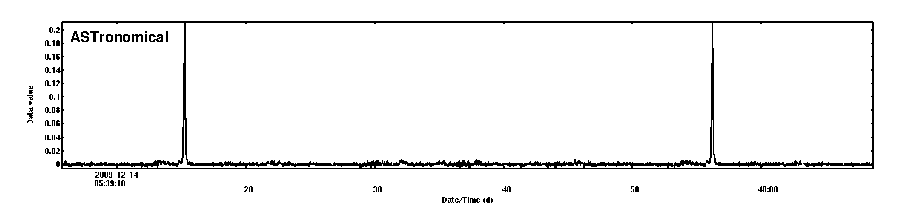
\includegraphics[width=\linewidth]{sc19_iter_ast} \\
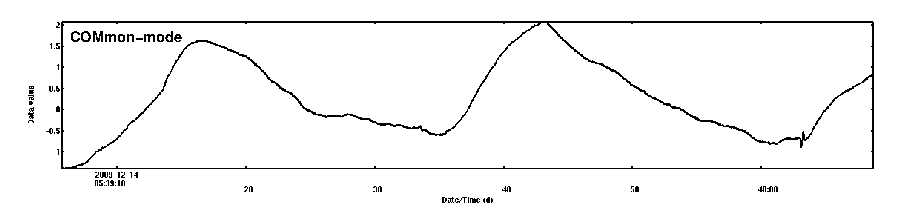
\includegraphics[width=\linewidth]{sc19_iter_com} \\
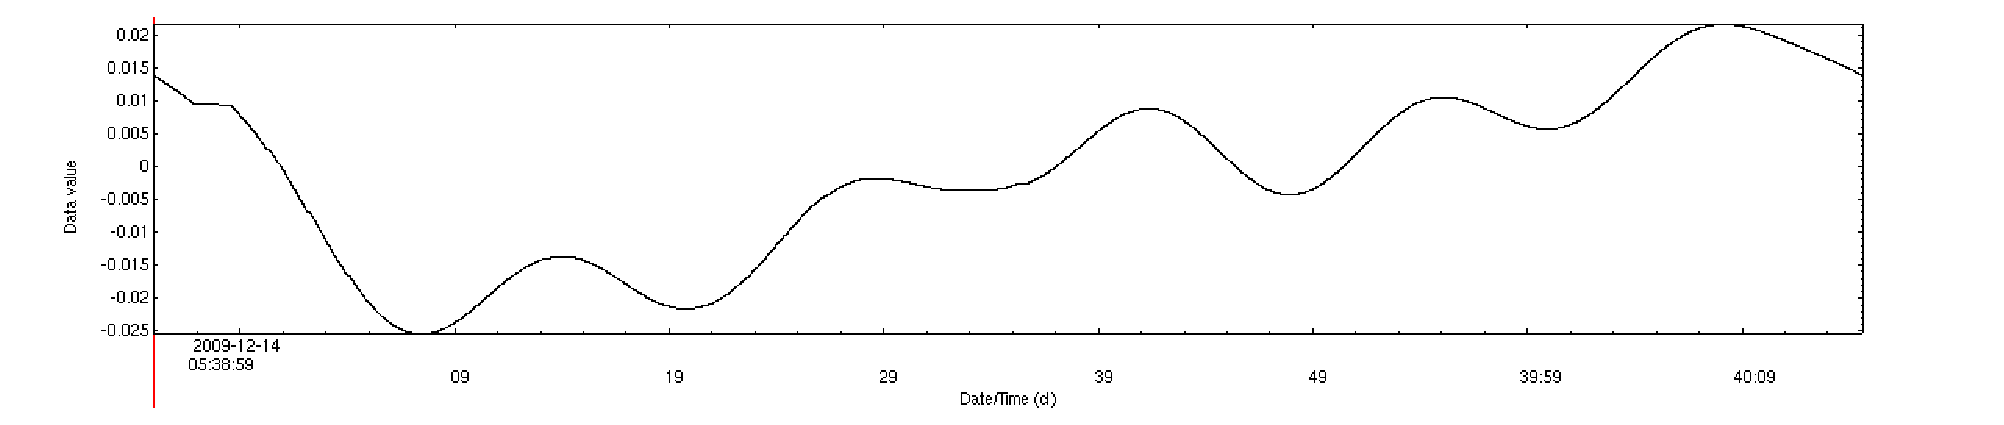
\includegraphics[width=\linewidth]{sc19_iter_flt} \\
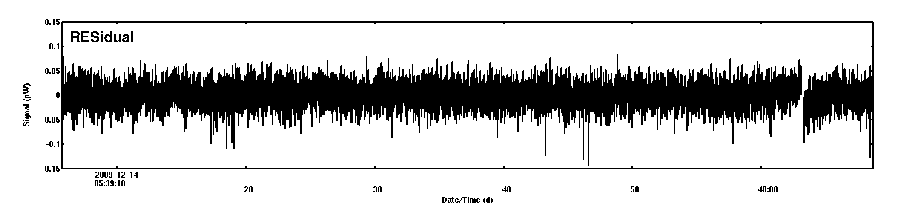
\includegraphics[width=\linewidth]{sc19_iter_res} \\
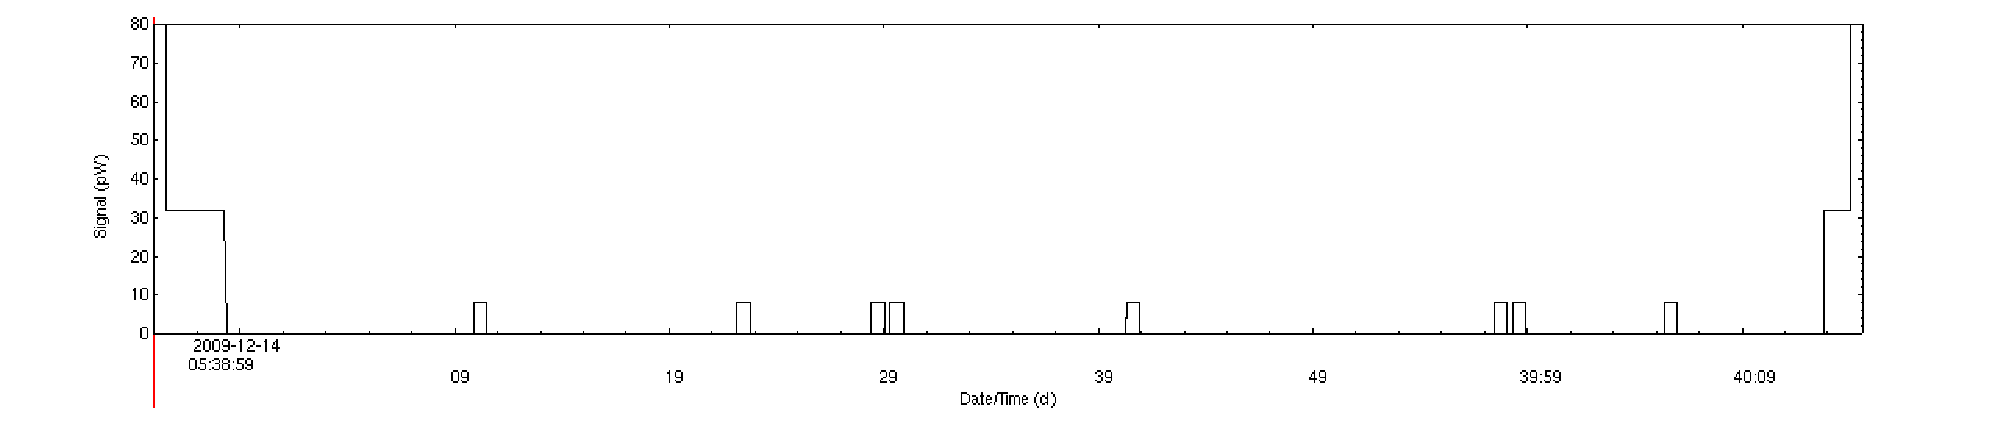
\includegraphics[width=\linewidth]{sc19_iter_qua} \\
\caption{Time-domain components of the iterative solution. From top to
  bottom: ASTronomical signal (clearly showing Uranus as positive
  spikes), COMmon mode (dominated by 30\,s fridge variations),
  FiLTered (residual low-frequency noise missed by COM), RESidual
  (looking flat and white as expected), and QUAlity (indicating
  padding/apodization at the start/end of the data, as well as 8 DC
  steps -- the numerical value 8). All of the figures (with the
  exception of the 1-d common-mode that was plotted with \Kappa\
  \linplot\ since it cannot be viewed with \gaia) were produced with
  \gaia.}
\label{fig:itercomp}
\end{center}
\end{figure}

Time traces for a single bolometer are compared for all of these model
components in Fig.~\ref{fig:itercomp}. Uranus is clearly seen as a
positive spike in the astronomical signal component. The common-mode
signal is the next largest, clearly exhibiting the 30\,s fridge
variations that are apparent in the raw data. The residual noise
removed by the high-pass filter is significant, but much smaller than
the common-mode component. Finally, the residual signal is quite flat,
indicating that most of the signal has been accounted for in the other
model components.

\section{\xlabel{calib}Calibrating SCUBA-2 Data}
\label{sec:calib}

\section{\xlabel{Examples}Examples of Different Reductions}
\label{sec:eg}

\subsection{\xlabel{Cosmology}Cosmology Data}
\label{sec:cosmology}

Deep cosmology observations are typically designed to detect
un-resolved high-redshift galaxies. Since the surface density of these
distant sources falls rapidly with increasing brightness, most objects
are, on average, only slightly brighter than the extra-galactic
confusion limit --- the flux density below which the surface density
of sources is so great that there are many blended objects within a
telescope beam. Consequently, the sources of interest are usually only
a few standard deviations brighter than the noise in the map (caused
by a combination instrumental and source confusion). In light of this,
the recommended strategy for reducing such maps involves two basic
steps:

\begin{enumerate}

\item Create a map using {\texttt dimmconfig\_blank\_field} which,
  compared to the default configuration, sacrifices structure on large
  scales to gain the best possible noise performance on small scales
  (i.e. making the map as flat as possible). This is a good compromise
  since the sources should generally be the size of a telescope beam.

\item Run the map through a combined `matched filter' (which
  effectively fits a PSF centered over every pixel in the map) and a
  background supression filter (removing additional residual
  large-scale noise). This is a fairly standard technique used
  throughout the extra-galactic submm community to identify potential
  sources.

\end{enumerate}

For this example we will reduce a 13 minute, 450\,\micron, $6' \times
6'$ CURVY\_PONG map towards the cluster MS0451. The data may be
retrieved from {\bf URL?}. Although not deep enough to detect any
individual sources, this example is useful to illustrate features that
are common to most of the extra-galactic SRO data from the Spring of
2010.

First, assuming the data are in the current directory, we produce a map
using the specialized {\texttt dimmconfig\_blank\_field}:

\begin{myquote}
\begin{verbatim}
% makemap s4a20100313_00029_00\*.sdf map450 method=iterate \
config=^$STARLINK_DIR/share/smurf/dimmconfig_blank_field.lis
\end{verbatim}
\end{myquote}

For comparison, we also make a map using the default configuration:

\begin{myquote}
\begin{verbatim}
% makemap s4a20100313_00029_00\*.sdf map450_default method=iterate \
config=^$STARLINK_DIR/share/smurf/dimmconfig.lis
\end{verbatim}
\end{myquote}

Both of the maps are shown in Fig.~\ref{fig:cosmomap}. Clearly the
specialized configuration for cosmology fields yields a flatter map,
although the white noise level is still quite large (no obvious
sources are visible), and there is some residual structure in the map
caused by low-frequency noise that is not effectively modelled/removed
by the map-maker (vertical stripes that are aligned with the map
edges).

\begin{figure}
\begin{center}
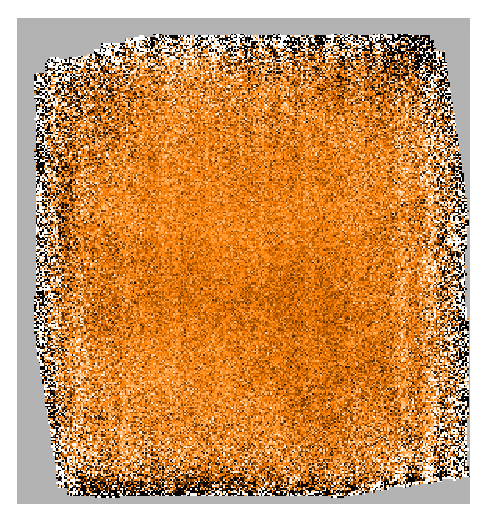
\includegraphics[width=0.49\linewidth]{sc19_cosmo_map}
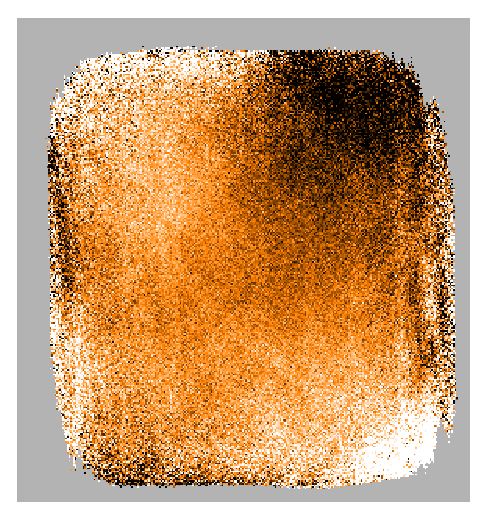
\includegraphics[width=0.49\linewidth]{sc19_cosmo_map_default} \\
\caption{Maps of a deep cosmology field, MS0451, at 450\,\micron. {\bf
    Left:} map using the specialized {\texttt
    dimmconfig\_blank\_field} which gives a significantly flatter
  result than {\bf Right:} map using the default {\texttt
    dimmconfig}.}
\label{fig:cosmomap}
\end{center}
\end{figure}

In order to optimally find sources that are the size of the telescope
beam, and suppress this residual large-scale noise, we provide a
script called {\texttt matched-filter}.

If there were no large-scale noise in the map, the filtered signal map
would be calculated as follows:
%
\begin{equation}
\mathcal{M} = \frac{[M(x,y)/\sigma^2(x,y)] \otimes P(x,y)}
  {[1/\sigma^2(x,y)] \otimes [P^2(x,y)]}.
\end{equation}
%
where $M(x,y)$ and $\sigma(x,y)$ are the signal and RMS
noise maps produced by \smurf, and $P(x,y)$ is a map of the
PSF. `$\otimes$' denotes the 2-dimensional cross-correlation
operator. Similarly, the variance map would be calculated as
%
\begin{equation}
  \mathcal{N}^2 = \frac{1}{[1/\sigma^2(x,y)] \otimes [P^2(x,y)]}.
\end{equation}
%
This operation is equivalent to calculating the maximum-likelihood fit
of the PSF centered over every pixel in the map, taking into account
the noise. Presently $P$ is simply modelled as an ideal Gaussian
with a FWHM set to the diffraction limit of the telescope.

However, since there is large-scale (and therefore correlated from
pixel to pixel) noise, the script also has an additional step. It
first smooths the map by cross-correlating with a larger Gaussian
kernel to estimate the background, and then subtracts it from the
image. The same operation is also applied to the PSF to estimate the
effective shape of a point-source in this background-subtracted map.

Before applying the filter to our cosmology data, we first look at the
effect it has on the map of Uranus from Fig.~\ref{fig:itermap}. The script
is executed as follows:

\begin{myquote}
\begin{verbatim}
% $SMURF_DIR/matched-filter -np -s 15 uranus uranus_sm
\end{verbatim}
\end{myquote}
%
Here the `{\texttt -s 15}' flag indicates that the background should
be estimated by first smoothing the map and PSF with a $15''$ FWHM
Gaussian, and the `{\texttt -np}' flag indicates that the output map,
{\texttt uranus\_sm}, should be re-normalized such that the peak
fluxes of point sources are conserved. The result is shown in
Fig.~\ref{fig:cosmo_filt}.

\begin{figure}
\begin{center}
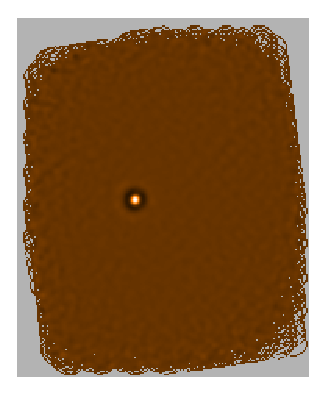
\includegraphics[width=0.46\linewidth]{sc19_uranus_filt}
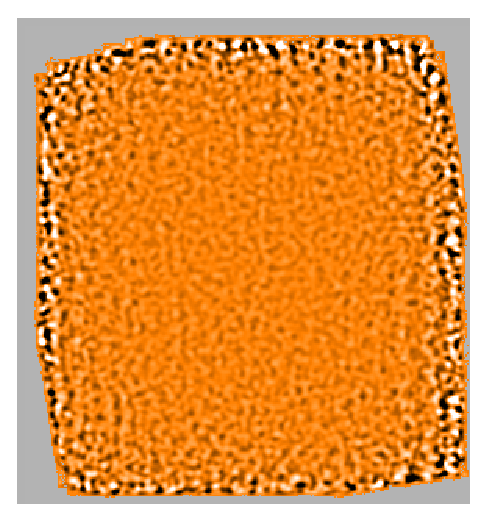
\includegraphics[width=0.525\linewidth]{sc19_cosmo_map_filt}
\caption{450\,\micron\ maps processed with the {\texttt
    matched-filter} script, suppressing scales larger than
  $15''$. {\bf Left:} filtered map of Uranus from
  Fig.~\ref{fig:itermap}. {\bf Righ:} filtered version of deep
  Cosmology map from left-hand panel of Fig.~\ref{fig:cosmomap}.}
\label{fig:cosmo_filt}
\end{center}
\end{figure}

The map is generally flatter, and the noise level is significantly
reduced. However, the price that we pay for suppressing signal on
scales larger that $15''$ is visible as the large negative ring around
the source; for this particular case the dip is about 10\% of the peak
signal.

Now that we know what this procedure does to a bright point source, we
proceed to filter the deep map. It is shown next to Uranus in
Fig.~\ref{fig:cosmo_filt}.

\begin{myquote}
\begin{verbatim}
% $SMURF_DIR/matched-filter -np -s 15 map450 map450_sm
\end{verbatim}
\end{myquote}

As hoped, this map has most of the remaining large-scale residual
structure removed, and in general the noise is significantly reduced.

Finally, how should we find sources? The filtered map also contains a
VARIANCE component, so it is easy to produce a S/N map using the \Kappa\
tasks \ndfcopy\ and \Div:

\begin{myquote}
\begin{verbatim}
% ndfcopy map450_sm map450_sm_noise comp=error
% div map450_sm map450_sm_noise map450_sm_snr
\end{verbatim}
\end{myquote}

The resulting map, {\texttt map450\_sm\_snr} is shown in
Fig.~\ref{fig:cosmo_snr}. Compared to Fig.~\ref{fig:cosmo_filt} the
edges no longer appear as noisy because they have been down-weighted
by the larger noise estimated there.

\begin{figure}
\begin{center}
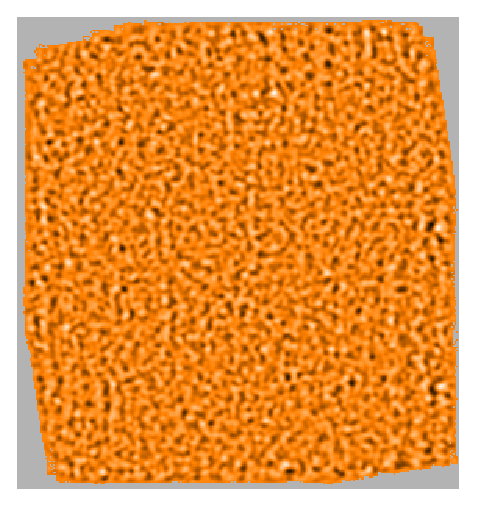
\includegraphics[width=0.49\linewidth]{sc19_cosmo_map_snr}
\caption{S/N map produced from the match-filtered deep cosmology map
  in Fig.~\ref{fig:cosmo_filt}, scaled from $-4\sigma$ (black) to
  $+4\sigma$ (white).}
\label{fig:cosmo_snr}
\end{center}
\end{figure}

A basic procedure for identifying sources would be to locate peaks
above some threshold S/N. However, as a word of caution, even after
all of these steps the noise may not be perfectly well-behaved. In
this example we do not expect any real astronomical source, so the S/N
map {\em should} have a brightness distribution that resembles a
Gaussian with standard deviation $\sigma=1$ and mean zero. We perform
this comparison for the central $100 \times 100$ pixels of the S/N map
in Fig.~\ref{fig:cosmo_snrcompare}, well away from any edge
effects. In this case we find that the real distribution is slightly
narrower than expected, suggesting that the noise has been
over-estimated.

\begin{figure}
\begin{center}
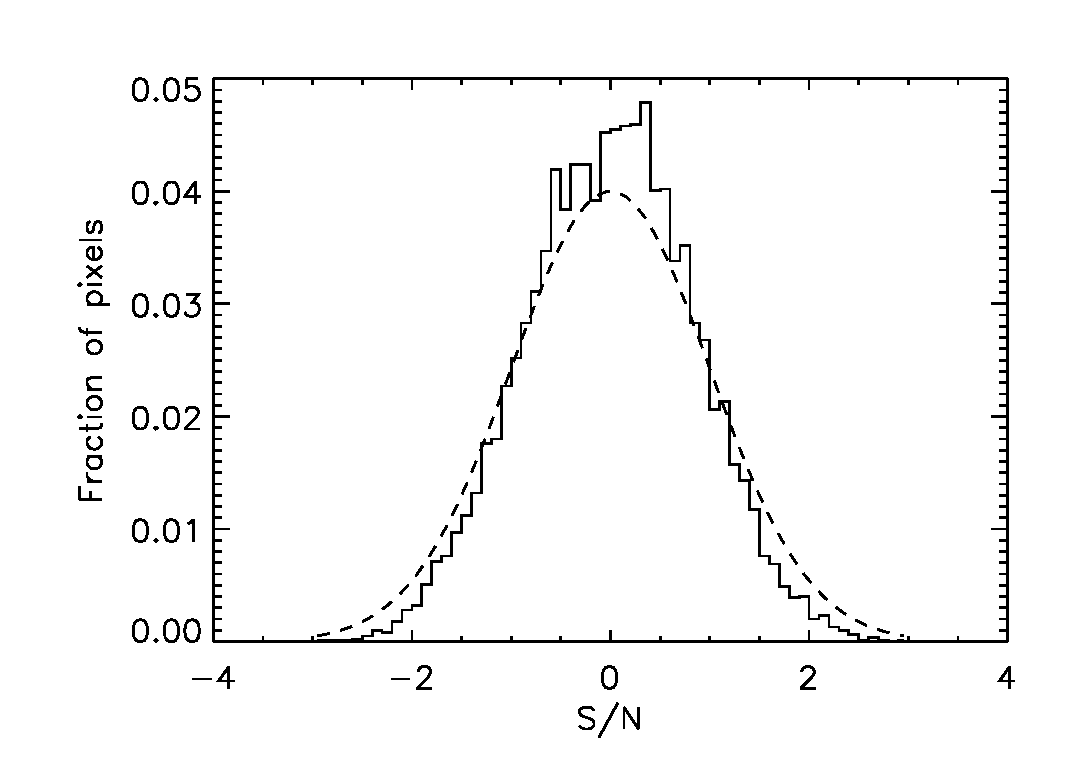
\includegraphics[width=0.8\linewidth]{sc19_cosmo_snrcompare}
\caption{The distribution of S/N for the central $100 \times 100$
  pixels of Fig.~\ref{fig:cosmo_filt} (histogram), compared with an
  ideal Gaussian distribution with mean zero and $\sigma=1$ (dashed
  line). The fact that the real distribution is skinnier demonstrates
  that in this region of the map the noise is probably slightly
  over-estimated.}
\label{fig:cosmo_snrcompare}
\end{center}
\end{figure}

We recognize that noise characterization is of utmost importance to
the deep Cosmology surveys, and we will continue to develop methods
for estimating the true noise distributions in the final maps (e.g.,
using Monte Carlo simulations). Also, the Gaussian background noise
suppression currently implemented in the matched-filter is
isotropic. Clearly some of the residual large-scale noise has a
preferred direction (such as the vertical stripes in
Fig.~\ref{fig:cosmomap}). We are therefore investigating ways of
automatically estimating more efficient filters for specific map
geometries that will hopefully result in flatter maps, with reduced
negative ringing around sources.

As a parting word on this subject, we mention some other tests that
PI's should consider undertaking:

\begin{itemize}

\item Split your data into mutually-exclusive subsets and produce
  independent maps. Are the highest S/N peaks detected in each of
  them?

\item Use {\em jackknife} tests to verify the estimated noise
  levels. Produce two maps from independent portions of the data and
  difference them (e.g., using the \Kappa\ task \sub). This will
  remove any astronomical signal, but increase the noise by a factor
  of about $\sqrt{2}$. Is the standard deviation in the central pixels
  (where the noise should hopefully be uniform) roughly $\sqrt{2}$
  larger than the noise estimated for either of the original maps?

\item How many {\em negative} peaks above a given S/N are there
  compared to the {\em positive} peaks?

\end{itemize}

\subsection{\xlabel{Galactic}Extended Galactic Sources}
\label{sec:galactic}

\begin{thebibliography}{}
\addcontentsline{toc}{section}{References}

\bibitem{smurf}
Chapin~E.~L., et~al., 2009, \textit{SMURF -- Sub-Millimetre User Reduction
Facility},
\xref{Starlink User Note 258}{sun258}{}

\bibitem{kappa}
Currie~M.~J., 1997, {\it KAPPA --- Kernel Application Package},
\xref{Starlink User Note 95}{sun95}{}

\bibitem{gaia}
Draper~P.~W., 1997, {\it GAIA -- Graphical Astronomy and Image
Analysis Tool},
\xref{Starlink User Note 214}{sun214}{}

\end{thebibliography}

\end{document}


